\documentclass[10pt,twocolumn,letterpaper]{article}
\usepackage[review]{cvpr}
%% Packages used by this paper (the CVPR 2027 kit loads booktabs, natbib, caption, subcaption and cleveref).
\usepackage{cuted}
\usepackage{multirow}
\usepackage{amsthm}
\newtheorem{proposition}{Proposition}
\AtBeginDocument{\crefname{proposition}{Prop.}{Props.}\Crefname{proposition}{Proposition}{Propositions}}

\definecolor{cvprblue}{rgb}{0.21,0.49,0.74}
\usepackage[pagebackref,breaklinks,colorlinks,allcolors=cvprblue]{hyperref}
\def\confName{CVPR}
\def\confYear{2027}
\newcommand{\relFaults}{138/138}
\newcommand{\relVacancies}{138/138}
\newcommand{\relAUC}{98.2}
\newcommand{\relAUCsrc}{48.6}
\newcommand{\relTopTwo}{77.5}
\newcommand{\relTopThree}{94.2}
\newcommand{\relThrR}{95.7}
\newcommand{\relThrW}{11.07}
\newcommand{\relListR}{97.1}
\newcommand{\relListW}{1.06}
\newcommand{\relPoolThrW}{4.58}
\newcommand{\relPoolThrR}{93.7}
\newcommand{\relPoolListW}{1.53}
\newcommand{\relPoolListR}{98.1}
\newcommand{\relAnyFault}{90.3}
\newcommand{\relAnyFaultX}{89.4}
\newcommand{\relAnyVacX}{2.8}
\newcommand{\relAnyShamX}{0.0}
\newcommand{\relAUCx}{98.2}
\newcommand{\relAnyVac}{2.9}
\newcommand{\relAnySham}{0.7}
\newcommand{\relArea}{5.4}
\newcommand{\relShamAlerts}{7}
\newcommand{\relSrcAlerts}{5}
\newcommand{\ppAny}{100.0}
\newcommand{\sbAny}{88.5}
\newcommand{\bbAny}{2.0}
\newcommand{\ppWaste}{14.6}
\newcommand{\fullSrcVal}{75}
\newcommand{\fullShamVal}{130}
\newcommand{\fullSrcX}{13}
\newcommand{\fullShamX}{64}
\newcommand{\scratchSentence}{\textbf{[pending]}}
\newcommand{\natPPrel}{33.9}
\newcommand{\natPPcw}{34.9 and 33.4}
\newcommand{\natPPfp}{78.5 and 71.6}
\newcommand{\natAddRel}{16.4}
\newcommand{\natAddFP}{83.7 and 70.1}
\newcommand{\cwSpread}{33.8 and 66.5}
\newcommand{\fpSpread}{1.6 and 1.4}
\newcommand{\cwThrW}{7.72 and 10.87}
\newcommand{\fpThrW}{4.57 and 6.15}
\newcommand{\fpPoolW}{1.09 and 3.36}
\newcommand{\cwPoolW}{2.85 and 5.34}
\newcommand{\fpTopThree}{89.1 and 80.4}
\newcommand{\dThrW}{3.2 [2.6, 3.8] and 4.7 [4.1, 5.4]}
\newcommand{\dSpread}{32 [26, 39] and 65 [58, 72]}
\newcommand{\fpShamAlerts}{25 and 6}
\newcommand{\cwShamAlerts}{19 and 15}
\newcommand{\natAddCW}{14.0 and 18.7}
\newcommand{\natMissRel}{45.2}
\newcommand{\natMissFP}{70.8 and 69.6}
\newcommand{\aucRel}{99.7}
\newcommand{\aucCW}{97.5 and 96.8}
\newcommand{\aucFP}{96.0 and 95.4}
\newcommand{\natSBrel}{17.6}
\newcommand{\natSBcw}{15.1 and 14.4}
\newcommand{\natSBfp}{15.4 and 15.6}
\newcommand{\natSBaddCW}{21.1}
\newcommand{\natSBaddFP}{0.0}
\newcommand{\sixFP}{71.6-$-$81.4}
\newcommand{\sixCW}{18.1-$-$34.9}
\newcommand{\sixMinGain}{38.2}
\newcommand{\eadRegFault}{92.9}
\newcommand{\eadRegAll}{69.4}
\newcommand{\eadSham}{128}
\newcommand{\eadSrc}{9}
\newcommand{\eadThrW}{0.21}
\newcommand{\eadShamQ}{1.28}
\newcommand{\pcRegFault}{84.3}
\newcommand{\pcRegAll}{66.4}
\newcommand{\pcSham}{123}
\newcommand{\pcSrc}{15}
\newcommand{\pcThrW}{0.82}
\newcommand{\pcShamQ}{1.86}
\newcommand{\relRegFault}{74.0}
\newcommand{\relRegAll}{81.6}
\newcommand{\relSham}{7}
\newcommand{\relSrc}{5}
\newcommand{\relShamQ}{0.00}
\newcommand{\ppRel}{33.9}
\newcommand{\ppCW}{34.9 and 33.4}
\newcommand{\ppFP}{78.5 and 71.6}
\newcommand{\ppGain}{+43.6 [26.6, 56.0] and +38.2 [16.5, 54.7]}
\newcommand{\bbRel}{18.3}
\newcommand{\bbCW}{18.2 and 18.5}
\newcommand{\bbFP}{27.2 and 30.7}
\newcommand{\bbGain}{+9.0 [4.2, 16.2] and +12.1 [6.9, 20.2]}
\newcommand{\sbRel}{17.6}
\newcommand{\sbCW}{15.1 and 14.4}
\newcommand{\sbFP}{15.4 and 15.6}
\newcommand{\sbGain}{+0.3 [$-$5.0, 2.6] and +1.2 [$-$2.1, 2.4]}
\newcommand{\jbRel}{33.6}
\newcommand{\jbCW}{39.5 and 38.3}
\newcommand{\jbFP}{39.4 and 38.4}
\newcommand{\jbGain}{$-$0.1 [$-$1.4, 1.9] and +0.0 [$-$1.5, 2.7]}
\newcommand{\scRel}{17.8}
\newcommand{\scCW}{18.0 and 23.6}
\newcommand{\scFP}{18.8 and 18.5}
\newcommand{\scGain}{+0.8 [$-$0.7, 4.8] and $-$5.1 [$-$11.9, 1.0]}
\newcommand{\ppAddGain}{+69.7 [47.4, 79.7] and +51.4 [21.0, 69.1]}
\newcommand{\bbCerealFP}{86.3 and 89.2}
\newcommand{\bbCerealCW}{60.0 and 54.7}
\newcommand{\opRelThrR}{51.0}
\newcommand{\opRelThrW}{5.3}
\newcommand{\opRelListR}{49.0}
\newcommand{\opRelListW}{1.1}
\newcommand{\opFPR}{76.2 and 80.5}
\newcommand{\opFPW}{1.9 and 3.1}
\newcommand{\opCWR}{54.4 and 77.3}
\newcommand{\opCWW}{4.5 and 5.1}
\newcommand{\opVsListR}{+27.2 [11.6, 40.1] and +31.4 [15.6, 43.7]}
\newcommand{\opVsListW}{+0.82 [0.34, 1.35] and +1.97 [1.24, 2.69]}
\newcommand{\opVsListClean}{$-$0.56 [$-$0.75, $-$0.37] and $-$0.41 [$-$0.62, $-$0.22]}
\newcommand{\opVsThrR}{+25.2 [10.2, 39.4] and +29.5 [14.1, 43.3]}
\newcommand{\opVsThrW}{$-$3.4 [$-$4.5, $-$2.2] and $-$2.2 [$-$3.3, $-$1.1]}
\newcommand{\opVsCWW}{$-$2.6 [$-$3.6, $-$1.6] and $-$2.1 [$-$3.0, $-$1.2]}
\newcommand{\opFPScene}{91.2 and 92.3}
\newcommand{\opFPGood}{9.4 and 18.1}
\newcommand{\opRelGood}{22.5}
\newcommand{\bbAucRel}{79.0}
\newcommand{\bbAucCW}{78.6 and 78.3}
\newcommand{\bbAucFP}{77.4 and 78.2}
\newcommand{\sbAucRel}{90.8}
\newcommand{\sbAucCW}{86.8 and 86.0}
\newcommand{\sbAucFP}{88.8 and 83.0}
\newcommand{\sbExtraCW}{4.3 and 0.6}
\newcommand{\sbExtraFP}{0.0 and 0.0}
\newcommand{\sbExtraGain}{$-$4.3 [$-$16.8, $-$0.1] and $-$0.6 [$-$9.6, $-$0.0]}
\newcommand{\insPPCW}{89.5 and 76.6}
\newcommand{\insPPFP}{5.0 and 1.9}
\newcommand{\insSBCW}{88.0 and 42.6}
\newcommand{\insSBFP}{14.6 and 3.8}
\newcommand{\toyRel}{13}
\newcommand{\toyCW}{11}
\newcommand{\toyFP}{4}
\newcommand{\toySpreadRel}{13}
\newcommand{\toySpreadFP}{0}
\newcommand{\officialSentence}{We ran the unmodified official evaluation functions on full-resolution, bilinearly upsampled copies of 4 pushpin heads (released: 33.2 official, 33.9 ours; classwide: 34.3 official, 34.9 ours; footprint: 78.4 official, 78.5 ours; classwide (seed 2): 32.7 official, 33.4 ours). The two implementations differ by at most 0.7 points and rank the heads identically.}
\newcommand{\scrSeeds}{2}
\newcommand{\scrSpreadCW}{25.4 and 97.9}
\newcommand{\scrSpreadFP}{1.8 and 1.6}
\newcommand{\scrThrWCW}{12.02 and 11.45}
\newcommand{\scrThrWFP}{0.24 and 0.59}
\newcommand{\scrPoolFP}{0.21 and 0.48}
\newcommand{\scrSproCW}{29.7 and 44.1}
\newcommand{\scrSproFP}{93.4 and 81.7}
\newcommand{\scrOpR}{79.9 and 76.2}
\newcommand{\scrOpW}{0.11 and 0.35}
\newcommand{\scrAucCW}{96.6 and 99.8}
\newcommand{\scrAucFP}{99.6 and 96.7}
\newcommand{\scrGain}{+63.7 [43.0, 79.2] and +37.6 [19.9, 51.8]}
\newcommand{\scrVsListR}{+30.9 [17.8, 40.7] and +27.2 [11.4, 39.9]}
\newcommand{\scrVsListW}{$-$0.99 [$-$1.18, $-$0.78] and $-$0.75 [$-$0.97, $-$0.50]}
\newcommand{\scrDThrW}{$-$11.8 [$-$12.3, $-$11.3] and $-$10.9 [$-$11.5, $-$10.1]}
\newcommand{\scrShamFP}{36 and 35}
\newcommand{\scrSrcFP}{10 and 12}
\newcommand{\scrShamCW}{6 and 47}
\newcommand{\scratchEndpoints}{Seed 1: primary endpoint met (footprint minus class-wide wasted inspections $-$11.78 [$-$12.26, $-$11.26]); scene-recall guardrail met; target-recall guardrail met (96.7\% against 96.0\%); sham guardrail not met (36 against 6 valid-sham alarms); reproduction check failed (class-wide spread 24.3\% on the oracle path, cell AUROC 87.4\%). Seed 2: primary endpoint met (footprint minus class-wide wasted inspections $-$10.86 [$-$11.46, $-$10.14]); scene-recall guardrail met; target-recall guardrail met (94.6\% against 96.7\%); sham guardrail met (35 against 47 valid-sham alarms); reproduction check passed (class-wide spread 96.4\% on the oracle path, cell AUROC 97.1\%).}

\graphicspath{{figures/}}
\title{Right Alarm, Wrong Places:\\Footprint Labels Fix Where Logical Anomaly Maps Point}
\author{Anonymous CVPR submission}
\begin{document}
\maketitlesupplementary

\noindent Part A documents every analysis in the main paper. Part B preserves the record of the earlier rounds of this study: short fine-tunes of the released head, the juice-bottle label rule, and the graph audit that motivated the matched-edit design. All tables are generated from saved outputs by the scripts in the package.

\section*{Part A: analyses in the main paper}
\section{Order of analyses and what was registered}
\label{sec:supp_order}
The 138 test and 69 development pushpin photographs, their edits, the re-segmenting U-Net and the released-map results were fixed in earlier rounds (Part B). This round added the following.
\begin{itemize}\setlength\itemsep{1pt}
\item \emph{Registered before scoring.} A protocol (SHA-256 prefix \texttt{a1e0af83}) frozen before any new head was scored specifies a from-initialization replication of the label comparison with SALAD's full 70{,}000-step recipe (\cref{sec:supp_scratch}), the pooled-tray analysis and the full-system calibration diagnostic.
\item \emph{Descriptive analyses of saved maps.} Threshold, list and relative queues for the released and earlier fine-tuned heads.
\item \emph{Added during this round, not registered.} The identical-input continuations reported in the main paper, the native AU-sPRO and fixed-operating-point evaluation of real defects, the instance-insertion probe and the two appearance detectors. They use the same fixed splits and decision rules, and every head and seed that was trained is reported, including the categories where footprint labels do not help.
\end{itemize}

\section{Inspection definitions}
\label{sec:supp_defs}
\paragraph{Scene gate.} The scene cutoff is the 63rd smallest map maximum of the 69 unedited development trays (the split-conformal $\lceil 70\times0.9\rceil$ order statistic), and a tray alarms when its maximum is strictly greater. Under exchangeability this bounds the marginal false-alarm probability of a new normal tray by 10\%; it does not bound the realized rate on a particular test set.
\paragraph{Queues.} Compartments are the 15 cells of the registered tray grid, and a compartment's score is the maximum of the map inside it. Only an alarmed tray opens a queue. The threshold is the highest cutoff at which at least 95\% of development targets on alarmed trays are queued; the list length is the smallest $k$ with the same property (ties broken by compartment index); the relative cutoff is the largest $\alpha$ on a 0.001 grid with the same property. Pooled trays contain the 69 development relocations and the 69 development vacancies, and every parameter is refit on them. On real defects we use the pooled parameters of each head, because real trays have one or several faulty compartments.
\paragraph{Diagnostics.} Change statistics compare an edited map with its own source on the 13 compartments untouched by the relocation, for every edit, so the three edits are compared on identical cells. The cell analogue of low-FPR sPRO integrates target-compartment recall against the false-compartment rate up to 5\% and normalizes; ``fault'' uses the 13 untouched compartments of each faulty tray as negatives and ``all'' adds every compartment of the unedited source and the valid sham.

\section{Identical-input continuations}
\label{sec:supp_ft}
For each category and seed, one process loads the released composition weights, freezes the released reconstruction autoencoder, and copies the discriminative U-Net into a class-wide and a footprint arm. Both arms consume one prefetched stream of 1{,}600 SALAD steps. Each step takes the next map of a per-epoch permutation of the official good training maps and its clean copy, and with probability 1/2 applies one of the four pinned edit families with a uniformly drawn donor map. The loss is SALAD's $5\times$ sigmoid focal plus L1 on the discriminative map. Adam ($10^{-5}$, weight decay $10^{-5}$) runs with a tenfold decay at step 1{,}520, and the final weights are used. This matches the 800 synthetic edits and 3:1 clean-to-edited ratio of the earlier continuation of Part B. The arms differ only in the insertion target, and the receipts store the hash of the shared input sequence. In the released generator, an insertion's target covers a median of 16 times the pasted area (median of per-edit ratios over 204 replayed pushpin insertions; the medians of the two areas themselves are 19{,}800 and 416 pixels).

\section{Native AU-sPRO}
\label{sec:supp_native}
\paragraph{Rules.} We read the official MVTec LOCO evaluation code to fix three rules. (i) Each ground-truth file is one defect channel with a defect-specific saturation: $\min(\text{threshold},\text{area})$ pixels for absolute and $\text{threshold}\times\text{area}$ for relative saturation; the channel's sPRO at a threshold is $\min(\text{TP area}/\text{saturation},1)$. (ii) A false positive is a positive pixel outside every channel of its image, and the false-positive rate pools all good and anomalous test images. (iii) The area under the mean sPRO curve is integrated up to a maximum false-positive rate and divided by it. We apply these rules to the $256{\times}256$ maps: ground-truth channels are downsampled by nearest neighbour and absolute saturation thresholds are scaled by the area ratio. Thresholds are 3{,}001 quantiles of the negative pixels between the 85th and 100th percentile plus $\pm\infty$. Only logical anomalies and good images enter.
\paragraph{Agreement with the official evaluator.} \officialSentence
\paragraph{Intervals.} We resample the test images (good and anomalous) with replacement, 2{,}000 times, and recompute the pooled false-positive rate and mean sPRO on each draw; all heads use the same draws, so differences are paired.
\begin{table*}[t]
\centering
\caption{Native logical anomalies in every category with a retrained pair: AU-sPRO up to 5\% FPR (\%) with 95\% intervals, and image AUROC (\%).}
\label{tab:native_full}
\footnotesize\setlength{\tabcolsep}{3pt}
\begin{tabular}{lcccccrcc}
\toprule
Category & Released & Class-wide 1 & Class-wide 2 & Footprint 1 & Footprint 2 & \multicolumn{3}{c}{Image AUROC: rel. / cw. / fp.} \\
\midrule
Pushpins & 33.9 [19.8, 57.7] & 34.9 [23.7, 51.9] & 33.4 [18.1, 56.3] & 78.5 [66.4, 90.5] & 71.6 [59.6, 83.8] & 99.7 & 97.5 / 96.8 & 96.0 / 95.4 \\
Breakfast box & 18.3 [13.4, 22.8] & 18.2 [13.5, 23.1] & 18.5 [12.9, 23.6] & 27.2 [21.9, 33.2] & 30.7 [24.7, 37.2] & 79.0 & 78.6 / 78.3 & 77.4 / 78.2 \\
Juice bottle & 33.6 [29.8, 38.1] & 39.5 [35.0, 44.3] & 38.3 [34.1, 43.2] & 39.4 [35.0, 44.3] & 38.4 [34.5, 43.3] & 88.1 & 89.7 / 87.4 & 88.3 / 86.6 \\
Splicing conn. & 17.8 [12.6, 35.4] & 18.0 [14.6, 29.0] & 23.6 [16.4, 39.3] & 18.8 [15.4, 32.3] & 18.5 [15.2, 32.6] & 82.7 & 82.3 / 81.2 & 82.8 / 85.6 \\
Screw bag & 17.6 [13.6, 24.0] & 15.1 [11.2, 22.9] & 14.4 [11.1, 20.1] & 15.4 [12.0, 20.3] & 15.6 [12.0, 20.3] & 90.8 & 86.8 / 86.0 & 88.8 / 83.0 \\
\bottomrule
\end{tabular}

\end{table*}

\section{Real defects at fixed operating points}
\label{sec:supp_op}
A compartment of a real pushpin image is a target when the union of its ground-truth channels covers at least 20 of its pixels at $256{\times}256$. The scene cutoff, threshold and list length of each head are the pooled parameters fitted on the development trays (\cref{sec:supp_defs}); nothing is fitted on real defects. \Cref{tab:native_op} reports every head and both queue policies with 95\% intervals over test images.
\begin{table*}[t]
\centering
\caption{Real pushpin defects at development-fixed operating points: recall of defective compartments, intact compartments opened per anomalous image, compartments opened per good image, and scene alarm rates.}
\label{tab:native_op}
\footnotesize\setlength{\tabcolsep}{4pt}
\begin{tabular}{llccccc}
\toprule
Head & Queue & Recall (\%) & Waste per defect & Queue per good tray & \multicolumn{2}{c}{Scene alarms (\%): defect / good} \\
\midrule
Released & threshold & 51.0 [39.1, 65.5] & 5.27 [3.95, 6.64] & 0.00 [0.00, 0.00] & 100.0 & 22.5 \\
 & list & 49.0 [41.7, 60.4] & 1.10 [0.91, 1.27] & 0.67 [0.48, 0.88] &  &  \\
\midrule
Class-wide, seed 1 & threshold & 54.4 [43.3, 67.0] & 4.54 [3.33, 5.80] & 0.01 [0.00, 0.03] & 97.8 & 18.1 \\
 & list & 47.0 [39.2, 58.7] & 1.11 [0.92, 1.29] & 0.54 [0.36, 0.73] &  &  \\
\midrule
Class-wide, seed 2 & threshold & 77.3 [64.7, 88.7] & 5.14 [3.92, 6.37] & 0.05 [0.01, 0.10] & 92.3 & 6.5 \\
 & list & 48.4 [41.5, 58.3] & 1.81 [1.55, 2.06] & 0.26 [0.11, 0.43] &  &  \\
\midrule
Footprint, seed 1 & threshold & 76.2 [63.8, 87.3] & 1.92 [1.40, 2.49] & 0.12 [0.06, 0.18] & 91.2 & 9.4 \\
 & list & 46.2 [38.5, 57.7] & 0.95 [0.76, 1.11] & 0.28 [0.15, 0.44] &  &  \\
\midrule
Footprint, seed 2 & threshold & 80.5 [68.3, 91.2] & 3.07 [2.30, 3.83] & 0.26 [0.17, 0.37] & 92.3 & 18.1 \\
 & list & 56.4 [49.1, 66.5] & 2.43 [2.12, 2.73] & 0.91 [0.60, 1.23] &  &  \\
\bottomrule
\end{tabular}

\end{table*}

\section{Training from initialization}
\label{sec:supp_scratch}
\paragraph{Recipe.} We reproduce the composition part of the released SALAD training loop (\texttt{train\_salad.py}, commit \texttt{753ba94}). The autoencoder and discriminative U-Net are the released architectures, initialized from scratch with the seed. Each step takes the next map of a per-epoch random permutation of the official good training maps (372 for pushpins, 360 for screw bag) and a uniformly drawn donor map. With probability 1/2 one of the four released edit families is applied: Perlin-shaped relabeling, same-image component relabeling, rotated insertion of a donor component, or relabeling plus insertion. The batch is this map and its clean copy. The autoencoder reconstructs the clean map from the (possibly edited) input with the released multiclass focal loss ($\gamma=2$, class weights from the released \texttt{get\_weights}) plus the released Dice loss. The U-Net receives the one-hot input and the reconstruction and is trained with $5\times$ mean sigmoid focal loss plus mean L1 against the discriminative target. Both networks use Adam at $10^{-5}$ with weight decay $10^{-5}$ and a tenfold decay at step 66{,}500 of 70{,}000. The appearance branches of SALAD are trained jointly in the original code but share no parameters or targets with the composition branch, so training the composition branch alone leaves its gradients unchanged up to the random stream. The Perlin helper uses OpenCV rotation in place of the original \texttt{imgaug} rotation, as in the 800-step fine-tunes (\cref{sec:supp_ft800}).
\paragraph{The only difference between arms.} \texttt{copy\_label\_diff\_img} pastes a rotated donor component and returns the entire channel of its class after pasting as the target. The \emph{class-wide} arm uses that target, as released. The \emph{footprint} arm uses the pasted donor mask captured before the expansion. For relabel-plus-insertion the relabel mask is united with either insertion target. Perlin and relabel targets are identical in both arms.
\paragraph{Identical inputs.} For each seed, one process initializes the two networks once, copies them to both arms, and feeds both arms the same prefetched stream. We hash the full sequence of input maps, clean maps and both target sequences; the two arms of a seed share every hash by construction, and the receipts store them (\texttt{results/scratch/*/fit.json}).
\paragraph{Scoring.} Final checkpoints (step 70{,}000) are scored on the oracle and re-extracted maps of every development and test edit, on the official native test maps, and in the insertion probe. Scene and spatial cutoffs are fit on development before test maps are read, exactly as for every other head.
\paragraph{Pre-specified endpoints.} The protocol fixed the primary endpoint before any from-initialization head was scored. That endpoint is footprint minus class-wide wasted inspections at the 95\% training threshold on the re-segmented path, with a useful effect defined as at least one compartment fewer and an interval excluding zero. It also fixed guardrails on scene recall, achieved target recall and valid-sham alarms, and a reproduction check of the released behaviour by the class-wide arm. \scratchEndpoints
\paragraph{Results.} \Cref{tab:replication_supp} repeats the main-paper replication table for reference.
\begin{table*}[t]
\centering
\caption{Replication with the full recipe (copy of the main-paper table).}
\label{tab:replication_supp}
\small
\input{tables/replication.tex}
\end{table*}



\section{Instance-insertion probe}
\label{sec:supp_insertion}
For a category with a multi-instance part class we take every official validation (development) and test good part map and paste one intact instance of that class from an official training map. Donor instances are connected components of the class with an area in the interquartile range of training instances (pushpins, screw bag) or between 2{,}000 and 4{,}500 pixels (a single fruit in breakfast box, whose fruits usually merge into one region). The placement is drawn uniformly, using a hash of the file name, among positions where the whole donor lies on the substrate on which the class normally rests (compartment floor, bag, or the cereal side of the box), at least three pixels from existing instances of the class. Pushpins then have an extra pin in a compartment, screw bags an extra part, and breakfast boxes a fruit in the wrong compartment; all three violate the published rules. ``Same-class any'' is the fraction of untouched same-class instances whose map changes by at least 0.5 somewhere, ``same-class area'' the fraction of their pixels that do, and ``other classes'' the same fraction over pixels of the remaining part classes more than ten pixels from the paste. Splicing connectors were excluded because their contacts leave no free substrate for an extra instance.
\begin{table*}[t]
\centering
\caption{Instance-insertion probe on part maps (composition branch). Instance AUROC ranks the pasted instance against the untouched instances of its class.}
\label{tab:insertion}
\footnotesize\setlength{\tabcolsep}{4pt}
\begin{tabular}{llrrrrrr}
\toprule
Category & Head & $n$ & Detect (\%) & Instance AUROC & Same-class any & Same-class area & Other classes \\
\midrule
Pushpins & released & 138 & 100.0 & 94.3 & 100.0 & 94.7 & 0.1 \\
 & class-wide 1 & 138 & 99.3 & 96.4 & 89.5 & 50.1 & 0.0 \\
 & class-wide 2 & 138 & 96.4 & 67.5 & 76.6 & 62.6 & 0.0 \\
 & footprint 1 & 138 & 96.4 & 96.0 & 5.0 & 1.3 & 0.0 \\
 & footprint 2 & 138 & 89.9 & 87.0 & 1.9 & 0.2 & 0.0 \\
\midrule
Screw bag & released & 122 & 100.0 & 91.0 & 88.5 & 73.0 & 0.0 \\
 & class-wide 1 & 122 & 100.0 & 89.1 & 88.0 & 57.3 & 0.0 \\
 & class-wide 2 & 122 & 90.2 & 89.2 & 42.6 & 20.2 & 0.0 \\
 & footprint 1 & 122 & 100.0 & 89.6 & 14.6 & 0.3 & 0.0 \\
 & footprint 2 & 122 & 77.0 & 92.0 & 3.8 & 0.0 & 0.0 \\
\midrule
Breakfast box & released & 102 & 100.0 & 100.0 & 2.0 & 0.0 & 0.0 \\
\bottomrule
\end{tabular}

\end{table*}

\section{Appearance detectors}
\label{sec:supp_appearance}
\paragraph{EfficientAD.} SALAD's local appearance branch is an EfficientAD student--teacher--autoencoder \cite{batzner2024} with the released pushpin weights. We use the pinned normalization of the full-system run (Part B) and compute its normalized map on every development and test edit; the map depends on RGB only, so both input paths coincide.
\paragraph{PatchCore.} We implement PatchCore \cite{roth2022} with an ImageNet WideResNet-50-2, layer-2 and layer-3 features with $3{\times}3$ local averaging, layer-3 features upsampled to the layer-2 grid, a 1\% greedy coreset (3{,}809 patch features from the 372 official good training photographs, selected after a random projection to 128 dimensions), nearest-neighbour distances, bilinear upsampling to $256{\times}256$ and Gaussian smoothing with $\sigma=4$. Inputs are the same uncropped composites as for the other detectors. Its native logical AUROC on the official pushpin test split is 73.2\%. Of the sham trays each detector queues, the queue includes the sham's edited compartment in 120 of 121 (EfficientAD) and 123 of 123 (PatchCore).

\section{Full SALAD operating point}
\label{sec:supp_full}
Full SALAD is replayed with the released weights and pinned code (Part B). SALAD normalizes each branch with statistics from the official validation split; we add a split-conformal 10\% cutoff on the 69 unedited development trays, which is our operating point and not one published with SALAD. For the normal-test cutoff we fit the same rule on the unedited sources of one fixed half of the test trays and apply it to all edits of the other half, then swap halves and add the counts. On the re-segmented path, the Gaussian branch's median normalized score is $+0.06$ on validation and $+2.73$ on unedited test trays, with the same pattern on the oracle path. The other branches shift little, and the shift is present in native good test images.


\section*{Part B: record of earlier rounds}
\section{Short fine-tunes of the released head}
These experiments preceded the identical-input continuations of the main paper. They adapt the released composition U-Net for 800 steps with the reconstruction autoencoder frozen, either on SALAD's own edit families (``original edits'') or with an added rule-aware training variant (``rule-aware''), and compare class-wide with footprint insertion targets inside each recipe. \Cref{tab:factorial} summarizes the resulting $2{\times}2$ design.
\begin{table*}[t]
\centering
\caption{Training recipe $\times$ insertion label in 800-step fine-tunes of the released head (matched trays, re-segmented path; same columns as the main matched-tray table). Development cell AUROC below 90\% fails the locked competence check ($^\dagger$).}
\label{tab:factorial}
\footnotesize\setlength{\tabcolsep}{3pt}
\begin{tabular}{llrrrrrrrrrr}
\toprule
\multicolumn{2}{l}{Detector, insertion label} & \multicolumn{2}{c}{Alarms} & Spread & \multicolumn{2}{c}{Threshold} & \multicolumn{2}{c}{List} & Pooled & \multicolumn{2}{c}{Region area} \\
\cmidrule(lr){3-4}\cmidrule(lr){6-7}\cmidrule(lr){8-9}\cmidrule(lr){11-12}
 & & fault & sham & (\%) & $W$ & $R$ & $W$ & $R$ & $W$ & fault & all \\
\midrule
Released & class-wide & 138 & \textbf{7} & 89.4 & 11.07 & 95.7 & 1.06 & 97.1 & 4.58 & 74.0 & 81.6 \\
\midrule
Original edits & class-wide, seed 1$^\dagger$ & 138 & 17 & 96.5 & 12.01 & 96.4 & 13.00 & 100.0 & 5.89 & 73.5 & 76.1 \\
 & footprint, seed 1 & 138 & 20 & 1.5 & 7.74 & 95.3 & 2.07 & 96.7 & 0.87 & 82.6 & 88.1 \\
 & class-wide, seed 2 & 138 & 18 & 88.8 & 11.50 & 96.0 & 2.04 & 97.8 & 5.40 & 68.8 & 71.9 \\
 & footprint, seed 2 & 138 & 20 & 1.3 & 7.07 & 95.3 & 2.06 & 97.1 & 1.04 & 78.5 & 87.1 \\
\midrule
Rule-aware & class-wide, seed 1$^\dagger$ & 138 & 19 & 100.0 & 13.00 & 97.1 & 13.00 & 100.0 & 7.12 & 36.2 & 39.3 \\
 & footprint, seed 1 & 138 & 9 & \textbf{0.0} & \textbf{0.20} & 95.3 & \textbf{1.01} & 99.6 & \textbf{0.16} & 88.4 & \textbf{96.3} \\
 & class-wide, seed 2$^\dagger$ & 138 & 22 & 100.0 & 13.00 & 96.4 & 13.00 & 100.0 & 6.75 & 36.0 & 39.4 \\
 & footprint, seed 2 & 138 & 20 & \textbf{0.0} & 0.45 & 96.0 & 1.02 & 98.9 & 0.28 & 77.3 & 89.6 \\
\bottomrule
\end{tabular}

\end{table*}
\subsection{Paired discriminative fine-tunes}
\paragraph{Released label construction.}
We use release revision \texttt{753ba942025d2644c494a18c1fb4b60ae15332d5} and the released checkpoints \cite{fucka2025}. \texttt{copy\_label\_diff\_img} overwrites the donor footprint in the edited six-channel map, then sets both the discriminative mask and the function's reconstruction-mask return value to the entire resulting inserted class plane. \texttt{copy\_and\_change} takes the maximum of the same-image relabel mask and this insertion mask. The reconstruction-mask return is ignored by the released training loop. The actual reconstruction objective uses the clean source labels with multiclass focal and Dice. The discriminative objective is
\[
  5\,{\rm mean}_{p}{\rm FL}_{.25,2}(z_p,y_p)
  + {\rm mean}_{p}|\sigma(z_p)-y_p|.
\]
Here $\mathrm{FL}$ uses the default sigmoid-focal coefficients $\alpha=.25$ and $\gamma=2$. Both terms average uniformly over all batch pixels. No inverse-area reweighting is used. The footprint variant records the paste mask before class expansion and changes the insertion portion only. The original relabel target remains intact for the combined operation. Both arms share the Perlin perturbation with bilinear OpenCV rotation and the released rotated donor insertion and relabel functions. The entire autoencoder is frozen, so the clean reconstruction objective does not train either U-Net.

\paragraph{Training schedule and receipts.}
There are 372 normal training originals and 371 eligible rule-aware training edits. Four-slot batches use two sampled clean maps, one sampled SALAD-family edit, and one edit from the training photo pool. In the last slot the draw proportions for relocation, sham, and vacancy are $1/2$, $1/4$, and $1/4$. Four SALAD edit families are sampled uniformly. In the upstream-only follow-up, the fourth slot is replaced by its clean source, preserving every augmented slot, donor and transform from the matched run. The expected 3:1 clean-to-synthetic ratio matches the released loader after its extra clean copy. Adam uses weight decay $10^{-5}$. Rule-aware fine-tuning starts at $3{\times}10^{-5}$, and upstream-only continuation starts at $10^{-5}$. Both run 800 steps in batches of four and multiply the learning rate by 0.1 after step 760. We use the last checkpoint for seeds 3407 and 3419. Every consumed clean map, input map and binary target is verified against the pre-specified per-example digests. Initial checkpoint and minibatch sequence hashes agree within each pair. The target sequence hashes differ. The head replaces a released head of the same architecture at inference. It adds training, rule-aware edit construction and validation calibration.

\begin{table*}[t]
\centering
\caption{\textbf{Positive mask area in paired rule-aware training.} Positive counts are means over examples of each edit type on a $256{\times}256$ grid. The upstream-only follow-up uses identical upstream edit slots and replaces the task-edit slot with a clean map.}
\label{tab:area_v3}
\small
\begin{tabular}{llrrr}
\toprule
Seed & Input edit & Examples & Class-wide px & Footprint px \\
\midrule
1 & Clean & 1600 & 0.0 & 0.0 \\
1 & Combined & 205 & 28841.7 & 8885.4 \\
1 & Insert & 204 & 22838.7 & 1583.1 \\
1 & Perlin & 187 & 2670.3 & 2670.3 \\
1 & Relabel & 204 & 7852.4 & 7852.4 \\
1 & Relocate & 409 & 3822.8 & 460.9 \\
1 & Vacancy & 169 & 228.5 & 228.5 \\
1 & Valid Sham & 222 & 0.0 & 0.0 \\
\midrule
2 & Clean & 1600 & 0.0 & 0.0 \\
2 & Combined & 204 & 27599.0 & 9901.4 \\
2 & Insert & 194 & 21770.8 & 1477.1 \\
2 & Perlin & 203 & 2503.0 & 2503.0 \\
2 & Relabel & 199 & 7625.5 & 7625.5 \\
2 & Relocate & 420 & 3823.8 & 462.4 \\
2 & Vacancy & 195 & 231.4 & 231.4 \\
2 & Valid Sham & 185 & 0.0 & 0.0 \\
\bottomrule
\end{tabular}

\end{table*}

\begin{table*}[t]
\centering
\caption{\textbf{Rule-aware fine-tuning on oracle labels.} See the main inspection table for definitions and the extracted results. Source and sham counts are paired within originals.}
\label{tab:oracle_v3}
\small
\setlength{\tabcolsep}{4.5pt}
\begin{tabular}{lccccrrr}
\toprule
Map and cell score & Src. / Sham & Fault / Vac. & Top 2 (\%) & Marks to both & Recall (\%) & Untouched & Reg. area \\
\midrule
Released, max & 31 / 31 & 138 / 138 & 76.8 & 2.46 & 95.3 & 10.51 & 81.4 \\
Released, 99th pct. & 31 / 31 & 138 / 138 & 87.0 & 2.33 & 95.3 & 11.07 & 77.6 \\
\midrule
Class-wide, seed 1 & 16 / 24 & 138 / 138 & 1.4 & 14.81 & 96.0 & 13.00 & 39.9 \\
Footprint, seed 1 & 14 / 18 & 138 / 138 & 87.7 & 2.12 & 96.0 & 0.20 & 95.4 \\
\midrule
Class-wide, seed 2 & 22 / 29 & 138 / 138 & 1.4 & 14.81 & 96.0 & 13.00 & 40.2 \\
Footprint, seed 2 & 15 / 16 & 138 / 137 & 76.1 & 2.28 & 96.0 & 0.46 & 88.8 \\
\bottomrule
\end{tabular}

\end{table*}

\begin{table*}[t]
\centering
\caption{\textbf{Paired rule-aware differences at the pre-specified cutoffs.} Untouched is in marks per fault. Target recall, sham alerts and region area use percentage points. Each interval uses 4,000 resamples of original photographs.}
\label{tab:contrasts_v3}
\small
\begin{tabular}{llrrrr}
\toprule
Input & Footprint contrast & Untouched & Target recall & Sham alarm & Region area \\
\midrule
Extracted & Seed 1 vs. released & -10.88 [-11.56, -10.12] & -0.4 [-3.6, +3.3] & +1.4 [-3.6, +7.2] & +14.7 [+10.8, +18.6] \\
Extracted & Seed 1 vs. class-wide & -12.80 [-12.87, -12.72] & -1.8 [-4.7, +1.1] & -7.2 [-13.8, -0.0] & +57.0 [+53.5, +60.5] \\
Extracted & Seed 2 vs. released & -10.62 [-11.31, -9.86] & +0.4 [-2.9, +3.6] & +9.4 [+2.2, +16.7] & +8.0 [+3.3, +13.0] \\
Extracted & Seed 2 vs. class-wide & -12.55 [-12.65, -12.45] & -0.4 [-3.6, +2.9] & -1.4 [-9.4, +6.5] & +50.3 [+46.1, +54.6] \\
\midrule
Oracle & Seed 1 vs. released & -10.30 [-11.05, -9.49] & +0.7 [-2.5, +4.0] & -9.4 [-15.9, -2.9] & +14.0 [+9.9, +18.1] \\
Oracle & Seed 1 vs. class-wide & -12.80 [-12.86, -12.73] & +0.0 [-3.3, +2.9] & -4.3 [-11.6, +2.9] & +55.6 [+51.8, +59.2] \\
Oracle & Seed 2 vs. released & -10.04 [-10.80, -9.21] & +0.7 [-2.5, +4.0] & -10.9 [-19.6, -2.9] & +7.5 [+2.5, +12.6] \\
Oracle & Seed 2 vs. class-wide & -12.54 [-12.64, -12.42] & +0.0 [-3.3, +3.3] & -9.4 [-17.4, -1.4] & +48.7 [+44.3, +53.1] \\
\bottomrule
\end{tabular}

\end{table*}

\begin{table*}[t]
\centering
\caption{\textbf{Additional rule-aware operating points.} Top 3 is both targets at rank three. The 98\% and 0.5-cost cutoffs are set on development. Recalls and the fault-only low-FPR region area are percentages. Untouched, sham and vacancy-only costs are means per image. Sham marks and vacancy-only untouched marks use the 95\% development cutoff.}
\label{tab:operating_v3}
\scriptsize
\setlength{\tabcolsep}{3pt}
\begin{tabular}{llrrrrrrrr}
\toprule
Input & Policy & Top 3 & 98 rec. & 98 unt. & Cost rec. & Cost unt. & Fault region & Sham marks & Vac. unt. \\
\midrule
Extracted & Released, max & 94.2 & 98.9 & 12.56 & 81.9 & 0.30 & 74.0 & 0.00 & 0.39 \\
Extracted & Released, 99th pct. & 96.4 & 98.9 & 12.62 & 75.7 & 0.17 & 73.8 & 0.00 & 0.28 \\
Extracted & Released, 95th pct. & 92.8 & 98.6 & 12.46 & 73.2 & 0.25 & 73.2 & 0.00 & 0.11 \\
Extracted & Released, reconstruction product & 65.2 & 98.6 & 12.59 & 67.4 & 0.51 & 62.4 & 0.00 & 0.33 \\
Extracted & Class-wide, seed 1 & 0.0 & 97.5 & 13.00 & 39.5 & 0.65 & 36.2 & 0.43 & 1.37 \\
Extracted & Footprint, seed 1 & 99.3 & 97.5 & 0.22 & 100.0 & 0.38 & 88.4 & 0.01 & 0.14 \\
Extracted & Class-wide, seed 2 & 0.0 & 97.8 & 13.00 & 39.1 & 0.64 & 36.0 & 0.09 & 0.59 \\
Extracted & Footprint, seed 2 & 97.8 & 98.2 & 0.57 & 98.2 & 0.57 & 77.3 & 0.14 & 0.23 \\
\midrule
Oracle & Released, max & 92.8 & 98.2 & 12.32 & 83.0 & 0.39 & 72.7 & 0.12 & 0.37 \\
Oracle & Released, 99th pct. & 96.4 & 98.9 & 12.60 & 75.4 & 0.25 & 71.9 & 0.11 & 0.28 \\
Oracle & Released, 95th pct. & 91.3 & 98.6 & 12.51 & 73.6 & 0.39 & 69.8 & 0.11 & 0.11 \\
Oracle & Released, reconstruction product & 69.6 & 98.9 & 12.64 & 71.7 & 0.41 & 67.1 & 0.12 & 0.40 \\
Oracle & Class-wide, seed 1 & 1.4 & 98.9 & 13.00 & 38.8 & 0.43 & 36.5 & 0.66 & 1.14 \\
Oracle & Footprint, seed 1 & 100.0 & 97.8 & 0.26 & 99.6 & 0.30 & 88.2 & 0.04 & 0.17 \\
Oracle & Class-wide, seed 2 & 1.4 & 98.9 & 13.00 & 38.4 & 0.42 & 35.9 & 0.38 & 0.84 \\
Oracle & Footprint, seed 2 & 96.4 & 98.9 & 0.64 & 98.2 & 0.58 & 77.9 & 0.13 & 0.23 \\
\bottomrule
\end{tabular}

\end{table*}

\begin{table*}[t]
\centering
\caption{\textbf{Descriptive equal-cost follow-up on extracted test faults.} Compare recall at two exact realized costs in untouched marks per image by interpolating the common-threshold sweep. Gains are against the released maximum in percentage points. Intervals resample the same original photos across readouts. The scene gate passes every fault in these rows. The development-pre-specified comparison remains the prospective decision test.}
\label{tab:exactcost}
\scriptsize
\setlength{\tabcolsep}{4pt}
\begin{tabular}{lrrrr}
\toprule
Readout & Recall at 0.30 & Gain & Recall at 0.50 & Gain \\
\midrule
Released, max & 81.9 [77.5, 85.5] & +0.0 [+0.0, +0.0] & 82.6 [79.0, 86.6] & +0.0 [+0.0, +0.0] \\
Released, 99th pct. & 77.5 [73.2, 81.5] & -4.3 [-7.2, -1.8] & 77.9 [73.6, 81.9] & -4.7 [-7.6, -2.5] \\
Footprint, seed 1 & 99.6 [96.7, 100.0] & +17.8 [+13.4, +22.1] & 100.0 [100.0, 100.0] & +17.4 [+13.4, +21.0] \\
Footprint, seed 2 & 88.4 [64.9, 96.0] & +6.5 [-16.7, +15.6] & 97.1 [94.2, 99.6] & +14.5 [+9.8, +18.8] \\
\bottomrule
\end{tabular}

\end{table*}

\subsection{Closer continuation of the released training recipe}
The two rule-aware class-wide heads detect the faults and vacancies but their localization fails the competence check. We therefore report a separately pre-specified continuation using only the original synthetic families in the augmented slot. The released head is the untouched reference. A paired effect here identifies target policy during this continuation. An end-to-end counterfactual of the released model would also refit the reconstruction network and start before the original 70,000-step training schedule. Positive area remains a component of the intervention.
A separately locked continuation uses the original synthetic edit families alone. Its class-wide seed 2 passes training competence (97.3\% extracted compartment AUROC), ranks targets at 98.1\% test AUROC and produces a large change in 88.8\% of untouched compartments. In that pair, footprint supervision reduces the fraction to 1.3\% and the queue from 11.50 to 7.07, a paired reduction of 4.43 marks [3.72, 5.14] at 96.0\% and 95.3\% target recall. Both heads detect all faults and vacancies, with 18 and 20 sham alarms. Seed 1 gives a similar queue reduction and misses the training AUROC floor. This isolates an effect of insertion targets during a continuation that reproduces the broad response in one competent control. The fine-tune with rule-aware examples achieves the lowest queues.


\begin{table*}[t]
\centering
\caption{\textbf{Upstream-only continuation on extracted maps.} The original SALAD-style augmentations are used without explicit relocation targets from the pushpin rule. Scene alerts and spatial metrics have the same definitions as the main table.}
\label{tab:upstream_e}
\small
\setlength{\tabcolsep}{4pt}
\begin{tabular}{lccccrrr}
\toprule
Map and cell score & Src. / Sham & Fault / Vac. & Top 2 (\%) & Marks to both & Recall (\%) & Untouched & Reg. area \\
\midrule
Released, max & 5 / 7 & 138 / 138 & 77.5 & 2.43 & 95.7 & 11.07 & 81.6 \\
\midrule
Class-wide, seed 1 & 15 / 17 & 138 / 138 & 71.0 & 4.83 & 96.4 & 12.01 & 76.1 \\
Footprint, seed 1 & 18 / 20 & 138 / 138 & 76.8 & 2.56 & 95.3 & 7.74 & 88.1 \\
\midrule
Class-wide, seed 2 & 18 / 18 & 138 / 138 & 75.4 & 2.49 & 96.0 & 11.50 & 71.9 \\
Footprint, seed 2 & 23 / 20 & 138 / 138 & 71.7 & 2.57 & 95.3 & 7.07 & 87.1 \\
\bottomrule
\end{tabular}

\end{table*}

\begin{table*}[t]
\centering
\caption{\textbf{Upstream-only continuation on oracle labels.} The released oracle path is shown for comparison.}
\label{tab:upstream_o}
\small
\setlength{\tabcolsep}{4pt}
\begin{tabular}{lccccrrr}
\toprule
Map and compartment score & Src. / Sham & Fault / Vac. & Top 2 (\%) & Marks to both & Recall (\%) & Untouched & Reg. area \\
\midrule
Released, max & 31 / 31 & 138 / 138 & 76.8 & 2.46 & 95.3 & 10.51 & 81.4 \\
\midrule
Class-wide, seed 1 & 16 / 20 & 138 / 138 & 60.9 & 5.02 & 96.7 & 12.08 & 73.7 \\
Footprint, seed 1 & 21 / 26 & 138 / 138 & 77.5 & 2.50 & 95.3 & 7.05 & 88.1 \\
\midrule
Class-wide, seed 2 & 24 / 30 & 138 / 138 & 77.5 & 2.43 & 97.1 & 11.75 & 71.9 \\
Footprint, seed 2 & 11 / 13 & 138 / 138 & 71.0 & 2.54 & 97.1 & 8.04 & 86.6 \\
\bottomrule
\end{tabular}

\end{table*}

\begin{table*}[t]
\centering
\caption{\textbf{Paired differences in the upstream-only continuation.} Untouched marks per fault and percentage-point differences at pre-specified cutoffs.}
\label{tab:upstream_diff}
\small
\begin{tabular}{llrrrr}
\toprule
Input & Footprint contrast & Untouched & Target recall & Sham alarm & Region area \\
\midrule
Extracted & Seed 1 vs. released & -3.33 [-3.90, -2.78] & -0.4 [-1.8, +0.7] & +9.4 [+3.6, +15.9] & +6.6 [+4.5, +8.8] \\
Extracted & Seed 1 vs. class-wide & -4.28 [-4.93, -3.66] & -1.1 [-2.9, +0.7] & +2.2 [-4.3, +8.7] & +12.1 [+8.8, +15.5] \\
Extracted & Seed 2 vs. released & -4.01 [-4.65, -3.34] & -0.4 [-2.2, +1.4] & +9.4 [+3.6, +15.9] & +5.5 [+3.5, +7.7] \\
Extracted & Seed 2 vs. class-wide & -4.43 [-5.14, -3.72] & -0.7 [-2.2, +0.7] & +1.4 [-3.6, +6.5] & +15.1 [+11.7, +18.5] \\
\midrule
Oracle & Seed 1 vs. released & -3.46 [-3.99, -2.95] & +0.0 [-1.1, +1.1] & -3.6 [-10.9, +3.6] & +6.8 [+4.6, +9.1] \\
Oracle & Seed 1 vs. class-wide & -5.03 [-5.67, -4.41] & -1.4 [-2.9, -0.4] & +4.3 [-2.9, +11.6] & +14.4 [+11.0, +18.1] \\
Oracle & Seed 2 vs. released & -2.46 [-3.00, -1.95] & +1.8 [+0.0, +3.6] & -13.0 [-19.6, -6.5] & +5.2 [+3.1, +7.5] \\
Oracle & Seed 2 vs. class-wide & -3.71 [-4.39, -3.09] & +0.0 [-1.4, +1.4] & -12.3 [-20.3, -5.1] & +14.7 [+11.6, +17.9] \\
\bottomrule
\end{tabular}

\end{table*}

\begin{table*}[t]
\centering
\caption{\textbf{Upstream-only alternate operating points.} Recalls and region area in percent. Counts are marks per photo. The released 99th percentile, 95th percentile and reconstruction product results appear in \cref{tab:operating_v3}.}
\label{tab:upstream_alt}
\scriptsize
\setlength{\tabcolsep}{3pt}
\begin{tabular}{llrrrrrrrr}
\toprule
Input & Policy & Top 3 & 98 rec. & 98 unt. & Cost rec. & Cost unt. & Fault region & Sham marks & Vac. unt. \\
\midrule
Extracted & Released, max & 94.2 & 98.9 & 12.56 & 81.9 & 0.30 & 74.0 & 0.00 & 0.39 \\
Extracted & Class-wide, seed 1 & 72.5 & 98.6 & 12.67 & 73.9 & 0.33 & 73.5 & 0.00 & 0.25 \\
Extracted & Footprint, seed 1 & 88.4 & 99.6 & 12.74 & 89.5 & 0.74 & 82.6 & 0.09 & 0.48 \\
Extracted & Class-wide, seed 2 & 92.0 & 99.6 & 12.64 & 70.3 & 0.21 & 68.8 & 0.01 & 0.46 \\
Extracted & Footprint, seed 2 & 87.7 & 99.3 & 11.28 & 87.7 & 0.60 & 78.5 & 0.18 & 1.95 \\
\midrule
Oracle & Released, max & 92.8 & 98.2 & 12.32 & 83.0 & 0.39 & 72.7 & 0.12 & 0.37 \\
Oracle & Class-wide, seed 1 & 68.1 & 97.1 & 12.34 & 71.0 & 0.20 & 70.9 & 0.12 & 0.23 \\
Oracle & Footprint, seed 1 & 92.8 & 98.6 & 12.33 & 88.4 & 0.51 & 82.7 & 0.17 & 0.39 \\
Oracle & Class-wide, seed 2 & 94.9 & 99.3 & 12.55 & 69.9 & 0.19 & 68.1 & 0.12 & 0.49 \\
Oracle & Footprint, seed 2 & 89.1 & 98.9 & 11.83 & 88.0 & 0.46 & 78.6 & 0.16 & 2.14 \\
\bottomrule
\end{tabular}

\end{table*}

\begin{table*}[t]
\centering
\caption{\textbf{Development controls and inspection thresholds.} Cell AUROC is measured on matched development faults. $t_s$ is the scene threshold. $t_{95}$ and $t_{98}$ use 95\% and 98\% target recall, and $t_{\rm budget}$ uses 0.5 untouched cells. Numbers are rounded for display. All decisions use full-precision thresholds.}
\label{tab:thresholds_v3}
\scriptsize
\setlength{\tabcolsep}{3.5pt}
\begin{tabular}{lllrrrrr}
\toprule
Input & Recipe & Readout & Dev. comp. AUC & $t_s$ & $t_{95}$ & $t_{98}$ & $t_{\rm budget}$ \\
\midrule
Extracted & Release & max & 97.9 & 0.17097 & 0.58810 & 0.30395 & 0.94571 \\
Extracted & Release & 99th pct. & 97.6 & 0.17097 & 0.40509 & 0.17635 & 0.91538 \\
Extracted & Release & 95th pct. & 98.2 & 0.17097 & 0.24504 & 0.10780 & 0.82902 \\
Extracted & Release & reconstruction product & 86.6 & 0.17097 & 0.40084 & 0.24098 & 0.85666 \\
Extracted & Rule-aware & Class-wide, seed 1 & 48.2 & 0.23692 & 0.24065 & 0.23530 & 0.99175 \\
Extracted & Rule-aware & Footprint, seed 1 & 99.6 & 0.15256 & 0.22907 & 0.21939 & 0.17743 \\
Extracted & Rule-aware & Class-wide, seed 2 & 48.6 & 0.16523 & 0.23033 & 0.21716 & 0.99440 \\
Extracted & Rule-aware & Footprint, seed 2 & 99.2 & 0.25479 & 0.24676 & 0.22138 & 0.22036 \\
\midrule
Oracle & Release & max & 98.3 & 0.15802 & 0.65622 & 0.38435 & 0.94875 \\
Oracle & Release & 99th pct. & 97.7 & 0.15802 & 0.48140 & 0.17617 & 0.92054 \\
Oracle & Release & 95th pct. & 97.8 & 0.15802 & 0.28629 & 0.10860 & 0.82870 \\
Oracle & Release & reconstruction product & 90.1 & 0.15802 & 0.39195 & 0.23391 & 0.86803 \\
Oracle & Rule-aware & Class-wide, seed 1 & 48.0 & 0.26617 & 0.22944 & 0.21414 & 0.99222 \\
Oracle & Rule-aware & Footprint, seed 1 & 99.3 & 0.14806 & 0.22603 & 0.21140 & 0.19119 \\
Oracle & Rule-aware & Class-wide, seed 2 & 48.8 & 0.16464 & 0.21921 & 0.19275 & 0.99473 \\
Oracle & Rule-aware & Footprint, seed 2 & 98.9 & 0.27966 & 0.23471 & 0.20151 & 0.21355 \\
\midrule
Extracted & Upstream-only & Class-wide, seed 1 & 86.3 & 0.12738 & 0.65216 & 0.45384 & 0.97235 \\
Extracted & Upstream-only & Footprint, seed 1 & 97.4 & 0.15104 & 0.14474 & 0.03827 & 0.39306 \\
Extracted & Upstream-only & Class-wide, seed 2 & 97.3 & 0.12330 & 0.52623 & 0.29629 & 0.97085 \\
Extracted & Upstream-only & Footprint, seed 2 & 97.9 & 0.13277 & 0.06335 & 0.02900 & 0.24583 \\
\midrule
Oracle & Upstream-only & Class-wide, seed 1 & 82.2 & 0.13064 & 0.67068 & 0.56927 & 0.97446 \\
Oracle & Upstream-only & Footprint, seed 1 & 97.7 & 0.15310 & 0.15520 & 0.05687 & 0.41723 \\
Oracle & Upstream-only & Class-wide, seed 2 & 97.4 & 0.12206 & 0.51133 & 0.29653 & 0.97182 \\
Oracle & Upstream-only & Footprint, seed 2 & 97.5 & 0.17490 & 0.05590 & 0.02490 & 0.26751 \\
\bottomrule
\end{tabular}

\end{table*}

\begin{table*}[t]
\centering
\caption{\textbf{Stability on two fixed photo halves.} Difference in untouched marks per fault, footprint minus class-wide. The 63 and 75 originals were assigned before fitting. The recipe with relocation training is the primary test. The upstream-only continuation reuses the same originals.}
\label{tab:halves_v3}
\scriptsize
\begin{tabular}{lllrr}
\toprule
Recipe & Input & Seed & Half A (63) & Half B (75) \\
\midrule
Rule-aware & Extracted & 1 & -12.87 [-12.95, -12.79] & -12.75 [-12.85, -12.63] \\
Rule-aware & Extracted & 2 & -12.63 [-12.76, -12.51] & -12.48 [-12.63, -12.32] \\
Rule-aware & Oracle & 1 & -12.86 [-12.94, -12.76] & -12.75 [-12.84, -12.64] \\
Rule-aware & Oracle & 2 & -12.54 [-12.68, -12.40] & -12.53 [-12.68, -12.37] \\
\midrule
Upstream-only & Extracted & 1 & -3.98 [-4.92, -3.14] & -4.52 [-5.41, -3.68] \\
Upstream-only & Extracted & 2 & -3.95 [-4.92, -3.02] & -4.84 [-5.81, -3.85] \\
Upstream-only & Oracle & 1 & -4.70 [-5.59, -3.87] & -5.31 [-6.19, -4.44] \\
Upstream-only & Oracle & 2 & -3.10 [-4.05, -2.21] & -4.23 [-5.12, -3.35] \\
\bottomrule
\end{tabular}

\end{table*}

\begin{table*}[t]
\centering
\caption{\textbf{Collateral change after rule-aware adaptation.} Cells and pixels report percentages with absolute change $\geq0.5$. Max and quantiles are mean within-cell statistics in sigmoid units. We use the same 13 untouched fault cells for each variant.}
\label{tab:changes_v3}
\scriptsize
\setlength{\tabcolsep}{4pt}
\begin{tabular}{lllrrrrr}
\toprule
Input & Policy & Edit & Cells (\%) & Pixels (\%) & Max & 99th pct. & 95th pct. \\
\midrule
Extracted & Released, max & Fault & 89.4 & 5.4 & 0.777 & 0.706 & 0.578 \\
Extracted & Released, max & Vacancy & 2.8 & 0.5 & 0.149 & 0.071 & 0.039 \\
Extracted & Released, max & Sham & 0.0 & 0.0 & 0.004 & 0.001 & 0.001 \\
Extracted & Class-wide, seed 1 & Fault & 100.0 & 6.5 & 0.980 & 0.970 & 0.868 \\
Extracted & Class-wide, seed 1 & Vacancy & 0.4 & 0.0 & 0.056 & 0.024 & 0.011 \\
Extracted & Class-wide, seed 1 & Sham & 0.2 & 0.0 & 0.013 & 0.006 & 0.003 \\
Extracted & Footprint, seed 1 & Fault & 0.0 & 0.0 & 0.053 & 0.015 & 0.005 \\
Extracted & Footprint, seed 1 & Vacancy & 0.0 & 0.0 & 0.017 & 0.007 & 0.004 \\
Extracted & Footprint, seed 1 & Sham & 0.0 & 0.0 & 0.002 & 0.000 & 0.000 \\
Extracted & Class-wide, seed 2 & Fault & 100.0 & 6.5 & 0.986 & 0.978 & 0.885 \\
Extracted & Class-wide, seed 2 & Vacancy & 0.2 & 0.0 & 0.035 & 0.015 & 0.006 \\
Extracted & Class-wide, seed 2 & Sham & 0.0 & 0.0 & 0.006 & 0.002 & 0.001 \\
Extracted & Footprint, seed 2 & Fault & 0.0 & 0.0 & 0.066 & 0.027 & 0.012 \\
Extracted & Footprint, seed 2 & Vacancy & 0.1 & 0.0 & 0.014 & 0.006 & 0.002 \\
Extracted & Footprint, seed 2 & Sham & 0.0 & 0.0 & 0.003 & 0.001 & 0.001 \\
\midrule
Oracle & Released, max & Fault & 90.3 & 5.4 & 0.781 & 0.711 & 0.578 \\
Oracle & Released, max & Vacancy & 2.9 & 0.6 & 0.152 & 0.075 & 0.043 \\
Oracle & Released, max & Sham & 0.7 & 0.5 & 0.010 & 0.007 & 0.006 \\
Oracle & Class-wide, seed 1 & Fault & 100.0 & 6.9 & 0.978 & 0.968 & 0.861 \\
Oracle & Class-wide, seed 1 & Vacancy & 0.8 & 0.5 & 0.052 & 0.023 & 0.012 \\
Oracle & Class-wide, seed 1 & Sham & 0.7 & 0.1 & 0.019 & 0.010 & 0.006 \\
Oracle & Footprint, seed 1 & Fault & 0.1 & 0.0 & 0.054 & 0.016 & 0.005 \\
Oracle & Footprint, seed 1 & Vacancy & 0.1 & 0.0 & 0.016 & 0.007 & 0.004 \\
Oracle & Footprint, seed 1 & Sham & 0.0 & 0.0 & 0.001 & 0.000 & 0.000 \\
Oracle & Class-wide, seed 2 & Fault & 100.0 & 6.5 & 0.983 & 0.975 & 0.876 \\
Oracle & Class-wide, seed 2 & Vacancy & 0.9 & 0.0 & 0.041 & 0.020 & 0.010 \\
Oracle & Class-wide, seed 2 & Sham & 0.2 & 0.0 & 0.010 & 0.005 & 0.004 \\
Oracle & Footprint, seed 2 & Fault & 0.0 & 0.0 & 0.067 & 0.027 & 0.012 \\
Oracle & Footprint, seed 2 & Vacancy & 0.1 & 0.0 & 0.012 & 0.005 & 0.002 \\
Oracle & Footprint, seed 2 & Sham & 0.0 & 0.0 & 0.003 & 0.001 & 0.001 \\
\bottomrule
\end{tabular}

\end{table*}

\begin{table*}[t]
\centering
\caption{\textbf{Collateral change after upstream-only continuation.} The region definition matches \cref{tab:changes_v3}.}
\label{tab:changes_upstream}
\scriptsize
\setlength{\tabcolsep}{4pt}
\begin{tabular}{lllrrrrr}
\toprule
Input & Policy & Edit & Cells (\%) & Pixels (\%) & Max & 99th pct. & 95th pct. \\
\midrule
Extracted & Released, max & Fault & 89.4 & 5.4 & 0.777 & 0.706 & 0.578 \\
Extracted & Released, max & Vacancy & 2.8 & 0.5 & 0.149 & 0.071 & 0.039 \\
Extracted & Released, max & Sham & 0.0 & 0.0 & 0.004 & 0.001 & 0.001 \\
Extracted & Class-wide, seed 1 & Fault & 96.5 & 6.3 & 0.889 & 0.848 & 0.705 \\
Extracted & Class-wide, seed 1 & Vacancy & 1.8 & 0.5 & 0.043 & 0.020 & 0.010 \\
Extracted & Class-wide, seed 1 & Sham & 0.1 & 0.0 & 0.008 & 0.004 & 0.003 \\
Extracted & Footprint, seed 1 & Fault & 1.5 & 0.0 & 0.171 & 0.061 & 0.022 \\
Extracted & Footprint, seed 1 & Vacancy & 0.9 & 0.0 & 0.024 & 0.009 & 0.003 \\
Extracted & Footprint, seed 1 & Sham & 0.0 & 0.0 & 0.003 & 0.001 & 0.000 \\
Extracted & Class-wide, seed 2 & Fault & 88.8 & 5.5 & 0.816 & 0.757 & 0.611 \\
Extracted & Class-wide, seed 2 & Vacancy & 2.7 & 0.5 & 0.100 & 0.048 & 0.020 \\
Extracted & Class-wide, seed 2 & Sham & 0.0 & 0.0 & 0.004 & 0.002 & 0.001 \\
Extracted & Footprint, seed 2 & Fault & 1.3 & 0.0 & 0.077 & 0.030 & 0.009 \\
Extracted & Footprint, seed 2 & Vacancy & 1.6 & 0.0 & 0.036 & 0.015 & 0.004 \\
Extracted & Footprint, seed 2 & Sham & 0.0 & 0.0 & 0.001 & 0.000 & 0.000 \\
\midrule
Oracle & Released, max & Fault & 90.3 & 5.4 & 0.781 & 0.711 & 0.578 \\
Oracle & Released, max & Vacancy & 2.9 & 0.6 & 0.152 & 0.075 & 0.043 \\
Oracle & Released, max & Sham & 0.7 & 0.5 & 0.010 & 0.007 & 0.006 \\
Oracle & Class-wide, seed 1 & Fault & 96.2 & 6.3 & 0.892 & 0.852 & 0.703 \\
Oracle & Class-wide, seed 1 & Vacancy & 1.8 & 0.5 & 0.042 & 0.021 & 0.012 \\
Oracle & Class-wide, seed 1 & Sham & 0.7 & 0.5 & 0.014 & 0.009 & 0.008 \\
Oracle & Footprint, seed 1 & Fault & 1.5 & 0.0 & 0.171 & 0.061 & 0.023 \\
Oracle & Footprint, seed 1 & Vacancy & 0.8 & 0.0 & 0.022 & 0.009 & 0.003 \\
Oracle & Footprint, seed 1 & Sham & 0.0 & 0.0 & 0.002 & 0.001 & 0.000 \\
Oracle & Class-wide, seed 2 & Fault & 90.4 & 5.5 & 0.817 & 0.760 & 0.608 \\
Oracle & Class-wide, seed 2 & Vacancy & 2.8 & 0.6 & 0.105 & 0.052 & 0.023 \\
Oracle & Class-wide, seed 2 & Sham & 0.7 & 0.5 & 0.011 & 0.008 & 0.007 \\
Oracle & Footprint, seed 2 & Fault & 1.4 & 0.0 & 0.077 & 0.030 & 0.009 \\
Oracle & Footprint, seed 2 & Vacancy & 1.6 & 0.0 & 0.034 & 0.014 & 0.004 \\
Oracle & Footprint, seed 2 & Sham & 0.0 & 0.0 & 0.001 & 0.000 & 0.000 \\
\bottomrule
\end{tabular}

\end{table*}


\section{Full fusion and the juice-bottle rule}
\subsection{Full fusion and a distinct liquid--label rule}
\paragraph{SALAD branch implementation.}
The released teacher, student, RGB autoencoder, map autoencoder and map U-Net are loaded from the same released archive. The RGB branch uses the released PIL resize and ImageNet normalization and uses only RGB in its local spatial map. The composition branch uses one-hot maps and a reconstruction. The Gaussian branch pools the first 384 channels of the RGB student over the full image and over semantic regions supplied by the maps. The implementation fits Ledoit--Wolf covariances on normal training features and applies validation means and standard deviations to the per-region distances. The feature statistics are refit on native normal train and validation RGB/map pairs. The official fusion sums the normalized local and map maxima and the released global score. Composition- and RGB-map spatial outputs are kept separately. We use normal-only 10\% alert cutoffs per tested branch and interface after applying the official normalizations. The extracted interface uses the same RGB and normalization statistics as the oracle route and substitutes maps from the audit's independent extractor. Our 91 native logical and 138 good pushpins reproduce the published 100.0\% full-system logical AUROC. On the matched photos the local RGB branch alerts on 128 valid shams, including 119 newly alerted from a clear source. Both edited arms retain the same cutout and paste support, so this is evidence of an appearance response to the composited valid move. Those shams are valid under the placement rule.

\begin{table*}[t]
\centering
\caption{\textbf{Released SALAD with all branches on the matched pushpins.} Strict normal-validation cutoffs, separately for each branch and interface. Wins give paired fault-over-sham direction with half ties. The global branch emits a scalar.}
\label{tab:fullpins}
\small
\begin{tabular}{llrrrrrr}
\toprule
Input & Branch & Source & Sham & Fault & Vacancy & New sham & Wins (\%) \\
\midrule
Oracle & Fusion & 77 & 131 & 138 & 138 & 54 & 100.0 \\
Oracle & Appearance & 9 & 128 & 138 & 137 & 119 & 78.3 \\
Oracle & Composition & 31 & 31 & 138 & 138 & 2 & 100.0 \\
Oracle & Global & 82 & 102 & 105 & 119 & 20 & 54.3 \\
\midrule
Extracted & Fusion & 75 & 130 & 138 & 138 & 55 & 100.0 \\
Extracted & Appearance & 9 & 128 & 138 & 137 & 119 & 78.3 \\
Extracted & Composition & 5 & 7 & 138 & 138 & 2 & 100.0 \\
Extracted & Global & 84 & 102 & 106 & 119 & 19 & 54.3 \\
\bottomrule
\end{tabular}

\end{table*}

\paragraph{Juice assets and eligibility.}
The dataset specifies a correspondence between the liquid and printed icon \cite{bergmann2022}. We use a fixed bank of 16 banana, 16 cherry and 16 orange donor photos from the official training split, sorted by a salted SHA-256 key among eligible cases. The upper and lower label windows are the two largest four-connected class-1 components. We place a $36{\times}56$ rectangle at the upper label's bounding-box center. At least 99.5\% of the rectangle must fall within the upper-label component. Liquid type is assigned by its exposed RGB median (a dark red channel below 105 for cherry, otherwise blue at least 90 for banana or at most 75 for orange). We inspected the source, donor and final icon crops before detector scoring. The RGB intervention leaves the original label border, lower label and bottle contents fixed. It retains the original composition map. The label identity is changed within the RGB print only.

The two donor crops use the same vertical offset from $\{-2,0,2\}$ and the same horizontal offset from $\{-8,-6,-4,0,4,6,8\}$ relative to their respective label centers. They must retain the icon's dark connected strokes within the unblended core. The original recipient rectangle and taper are shared. The taper reaches full opacity three pixels from its edge. Each donor border mean absolute difference is at most 13 digital levels, with a between-arm difference at most 2.5. Mean blended RGB differences between arms differ by at most 0.5 digital levels averaged over the recipient rectangle. The pair minimizes the sum of those matching gaps. A centered-crop feasibility pilot gave systematically greater edit magnitude for faults. The offset and core checks were set without model outputs. We retained 53/54 validation and 89/94 test sources. Reused donors are fixed assets. The original test photo is the bootstrap unit. Neither same-category pushpin half is counted as a new data domain.

\paragraph{Targets and results.}
We rank the local appearance map over upper label, lower label, cap, shoulder liquid and lower liquid. Among the 89 fault maps the upper label ranks first in 66 and has mean rank 1.33. It ranks first in 76/89 shams and 5/89 originals. With fusion as the scene gate, its development-calibrated spatial cutoff recovers it in 84/89 faults and queues 1.33 other regions per fault. Local appearance gives 28 sham and 25 fault scene alerts at its own cutoff. Fusion and global appearance each detect all 89 faults and order every fault above its sham. The exact binomial 95\% interval for an all-hit count is 95.9--100\%. The paired bootstrap intervals for the fault-minus-sham alert gaps are 70.8--87.6 points for fusion and 76.4--91.0 for global appearance. Composition-only yields the same output pixel for pixel across all variants, so any of its four scene alerts applies equally to each state.



\section{Graph audit}
\subsection{Refitted graph readout}
The mean-aggregation comparator uses the original query-masked endpoint inputs, message encoder, donor-balanced fitting loss and learning-rate and early-stop rules. It uses mean pooling within each neighborhood and the original mean/max pooling across the endpoints. It omits explicit degree inputs and degree-scaled pooling. Its original GlaS four folds yield normal-link AUROC between 95.7\% and 98.2\% with better loss than a prevalence intercept in all four. All 280 query-bit flip checks give exact equality. The mean model can still use neighborhood content that covaries with degree or recognize an empty neighborhood.

\begin{table*}[t]
\centering
\caption{\textbf{Response after refitting with mean aggregation.} AUC and top-four recovery use absolute matched probability change and donor-macro aggregation. Top-four change is refit minus original in percentage points. Intervals are donor-paired. The tiers share donors.}
\label{tab:refit}
\small
\begin{tabular}{lrrrr}
\toprule
Switch tier & Donors & Response AUROC & Top four & Top-four change \\
\midrule
Original & 12 & 91.5 [89.1, 93.7] & 46.6 [40.5, 52.4] & -40.9 [-49.8, -32.8] \\
Extra length-matched & 11 & 92.7 [90.1, 95.1] & 45.3 [40.2, 50.6] & -37.6 [-48.1, -23.0] \\
Joint-matched & 11 & 92.9 [90.3, 95.3] & 51.4 [41.7, 59.7] & -35.2 [-45.3, -25.6] \\
\bottomrule
\end{tabular}

\end{table*}

The original and refitted networks use a query-excluded adjacency for all tokens. A changed observed bit can affect a loss through the scoring formula without moving the fitted probability. The pair MLP is an invariance control because geometry and roles stay fixed. The degree-only probe concentrates its changed features on the four target pairs by construction. It tests whether the fitted model responds to that input. Its perfect recovery and the fixed-weight clamp should be interpreted with the refit in \cref{tab:refit}. SpotTarget studies degree-sensitive bias from including and excluding target edges \cite{zhu2024spot}. Our paired construction exposes a residual input difference after exclusion.

\clearpage

\subsection{Record of the earlier audit}
The following sections retain the earlier donor and switch experiments, released-model diagnostics, native LOCO analysis and clinical query. They document secondary and exploratory results and their original protocol. Claims about the earlier composition-only run refer to that run.

\subsection{Study and analysis scope}
We fixed the original GlaS and HVSMR graph folds and the existing MVTec LOCO partitions before fitting the new readouts. The original gland spacing decomposition was known. The earlier protocol froze the graph contrast, support rules, controls, and useful effect sizes before evaluating the new test scores. The earlier locked graph contrast was edited-state loss AUROC minus absolute probability-change AUROC, with a useful positive gap of at least ten points. The measured contrast reverses that direction. A fixed-model degree intervention was prompted by the test outcome and is exploratory. The visual test and the collateral response distribution use all eligible sources. The common-cell comparison of fault, sham, and deletion was a follow-up to the paired spatial output. The screw-bag extent and the native cardiac term probes are secondary follow-ups.

\paragraph{Paired estimands.}
All graph metrics compare four switch targets with the other pairs within the same graph. The fraction affected and magnitude summaries are computed separately on all targets, added edges, removed edges and untouched pairs. The two-hypothesis AUROC uses half credit for ties. Top-four recall uses fractional allocation to a tied boundary score. Within a source we first average its edits. Within a donor we then average its sources. Donors have equal aggregate weight. The paired bootstrap uses common draw indices across methods and metrics. For image edits, one original photograph and all its variants move together in resampling. Intervals condition on fitted checkpoints and validation cutoffs.

\subsection{Graph construction and matching}
GlaS provides 165 gland instance masks from 16 donors. We use the research-use mirror of the original Warwick-QU challenge files, the supplied donor IDs and $0.620\,\mu$m pixel spacing \cite{glas2017}. Graph adjacency is the undirected union of each gland's two closest annotated boundaries. The sensitivity construction takes the undirected union of its two closest centroids. HVSMR-2.0 uses cropped\_norm v2 in patient RAS axes. Each nonempty structure defines one typed node. Face contact of at least $5\,\mathrm{mm}^2$ defines a link \cite{pace2024}. Part features include log area or volume, elongation, compactness and channel intensity moments.

Of 165 GlaS fields, 140 have at least four nodes, 129 admit a switch, and 78 meet the original 1.35 length criterion. The 60 cardiac graphs all admit a switch and 59 meet the original bound. The saved manifest includes all original switch pairs. For extra edits we enumerate feasible degree-preserving switches on four distinct nodes and choose up to three distinct hash-ordered edits per source. The additional length tier excludes the saved edit. The alternate construction uses the same length criterion. The joint tier tries both assignments of the two additions to the two removals. It minimizes the maximum absolute log ratio across both raw and locally normalized lengths and requires both attributes to agree within a factor of 1.20. An exact role-pair match is prioritized within this bound. In cardiac graphs, each observed role is unique, so each unordered role pair identifies a single candidate. Matching the role-pair multiset exactly would fix the edge set. Cardiac joint switches are distance-matched. \Cref{tab:balance} reports the coverage tradeoff. The CRAG source paper describes an independent gland cohort \cite{graham2019mild}, but the obtainable tiles lacked a verified patch-to-donor key. All new gland edits and constructions therefore reuse GlaS donors.

\begin{table*}[t]
\centering
\caption{\textbf{Coverage, balance, and sensitivity to matching.} D/F/E gives donors, fields or scans, and edits. Raw and local columns give the median and maximum multiplicative imbalance under the \emph{same} correspondence. The original length criterion uses separately sorted raw lengths, so its maximum under the common correspondence can exceed 1.35. Roles counts exact role-pair matches. Gains are against typed centroid distance. Rank minus response compares the GNN's edited-state loss AUROC with its matched absolute probability-change AUROC. Paired intervals are in points.}
\label{tab:balance}
\scriptsize
\setlength{\tabcolsep}{3.5pt}
\begin{tabular}{@{}llrrrrrrr@{}}
\toprule
Cohort & Tier & D/F/E & Raw & Local & Roles & Local gain & Topol. gain & Rank $-$ response \\
\midrule
GlaS & All original & 14/129/129 & 1.18/5.66 & 1.19/6.71 & 258/258 & +11.8 [+8.9, +15.0] & -2.5 [-5.7, +0.8] & -10.5 [-14.4, -6.2] \\
GlaS & Centroid 2-NN & 11/64/120 & 1.21/1.87 & 1.19/1.60 & 240/240 & +15.4 [+11.0, +20.2] & +4.6 [+1.4, +8.1] & -5.1 [-7.1, -2.7] \\
GlaS & Extra length & 11/57/126 & 1.23/1.46 & 1.21/1.54 & 252/252 & +16.1 [+10.4, +22.4] & +4.5 [+0.5, +9.2] & -14.5 [-17.4, -11.7] \\
GlaS & Joint match & 11/36/48 & 1.08/1.20 & 1.08/1.20 & 96/96 & +16.8 [+11.3, +23.0] & +3.2 [-2.6, +9.6] & -17.1 [-22.8, -12.0] \\
GlaS & Original length & 12/78/78 & 1.11/1.58 & 1.10/1.52 & 156/156 & +15.3 [+10.9, +20.1] & +2.1 [-2.4, +7.1] & -16.0 [-19.9, -12.5] \\
\midrule
HVSMR & All original & 60/60/60 & 1.08/1.67 & 1.11/1.83 & 0/120 & +0.4 [-0.2, +1.0] & -5.3 [-6.4, -4.2] & -29.2 [-34.1, -23.8] \\
HVSMR & Extra length & 54/54/146 & 1.19/1.81 & 1.17/1.83 & 0/292 & +0.5 [-0.0, +0.9] & -4.4 [-5.6, -3.4] & -27.9 [-30.7, -24.9] \\
HVSMR & Joint match & 43/43/91 & 1.09/1.19 & 1.08/1.20 & 0/182 & +0.4 [-0.1, +1.0] & -4.2 [-5.4, -3.0] & -29.9 [-34.8, -24.9] \\
HVSMR & Original length & 59/59/59 & 1.08/1.67 & 1.11/1.83 & 0/118 & +0.4 [-0.2, +1.0] & -5.3 [-6.5, -4.1] & -29.5 [-34.5, -24.3] \\
\bottomrule
\end{tabular}

\end{table*}

\paragraph{An exact topology separation.}
Place four same-role parts at consecutive vertices of a unit square and two more at $(0.5,-0.8)$ and $(0.5,1.8)$, using the square from $(0,0)$ to $(1,1)$. Join each horizontal side to its adjacent exterior point to make two triangles. Replace the two horizontal links with the two vertical sides. The result is a six-cycle. Degrees are two in both states. All four switched links have raw length one, and all four square vertices have second-nearest centroid radius one. The multiset of roles, link state, raw distance, and local-normalized distance over all pairs is unchanged. A readout of this multiset must tie. Counting triangles or computing shared-neighbor evidence can distinguish the graphs. This construction isolates topology for this restricted representation.

\begin{table*}[t]
\centering
\caption{\textbf{Earlier graph ranking and response results.} Source and Edited rank targets by the observed-state anomaly score (geometry uses its fixed readout). Response ranks absolute change in conditional probability or change in the geometry readout. The edited intervals are donor paired. GlaS and HVSMR use 78 and 59 source graphs in the original length tier. The pair MLP and frozen GNN controls keep conditional probability fixed.}
\label{tab:previous_graph}
\scriptsize
\setlength{\tabcolsep}{3.5pt}
\begin{tabular}{@{}lrrr@{\hspace{10pt}}rrr@{}}
\toprule
 & \multicolumn{3}{c}{GlaS (78 fields, 12 donors)} & \multicolumn{3}{c}{HVSMR (59 scans, 59 donors)} \\
\cmidrule(lr){2-4}\cmidrule(l){5-7}
Readout & Source & Edited [95\% CI] & Response & Source & Edited [95\% CI] & Response \\
\midrule
Geometry only & 64.0 & 64.0 [57.1, 70.6] & 50.0 & 47.9 & 47.9 [43.4, 52.6] & 50.0 \\
Typed frequency & 61.8 & 61.8 [59.4, 64.2] & 50.0 & 62.4 & 84.5 [81.9, 86.9] & 50.0 \\
Typed distance & 70.1 & 74.9 [70.8, 78.9] & 50.0 & 64.7 & 87.3 [85.1, 89.5] & 50.0 \\
Distance + local spacing & 85.9 & 90.2 [88.4, 91.7] & 50.0 & 65.4 & 87.7 [85.6, 89.7] & 50.0 \\
Handcrafted full context & 80.6 & 85.8 [83.5, 88.0] & 99.3 & 61.2 & 83.5 [81.3, 85.7] & 96.5 \\
\midrule
Pair MLP & 86.7 & 91.5 [89.1, 93.6] & 50.0 & 68.4 & 80.4 [77.9, 83.1] & 50.0 \\
Masked GNN & 77.4 & 82.5 [78.3, 86.5] & 98.5 & 55.5 & 59.4 [56.8, 61.8] & 88.8 \\
GNN, context frozen & 77.4 & 96.2 [95.0, 97.3] & 50.0 & 55.5 & 88.5 [85.6, 91.1] & 50.0 \\
\bottomrule
\end{tabular}

\end{table*}

\subsection{Graph scorers and readout controls}
\paragraph{Fitting.}
Four test folds use the original hash-ordered donor allocation. For each family and fold we sort fitting donors by a second salted hash and take the first quarter, with a minimum of two, for development. The rest fit the two learned link models. Both use donor-balanced BCE, with the per-pair weight inversely proportional to the donor's field count and that field's candidate count. AdamW uses weight decay $0.002$ and batch size 512. Rates $0.002$ and $0.0007$ are compared using the smallest weighted development loss. We train up to 80 epochs with patience 12 and initial seeds 904--907. For GlaS there are nine fit and three development donors per fold. For HVSMR there are 34 and 11. Frozen logistic comparators retain all outer fitting donors and use the original $0.015$ regularization and feature scales.

\paragraph{Frozen references.}
Typed frequency uses add-one smoothing for the binary outcome within each unordered role pair. The typed centroid logit uses role-pair indicators, the log ratio of distance to the graph median distance, and the squared log-distance term. The log ratio is clipped to $[-5,3]$. Context adds the log local-spacing ratio, $\log(1+\mathrm{CN})$, Jaccard overlap, and the logs of one plus the smaller and larger masked degrees. Spacing and topology-only references select the corresponding context features. Feature scales are the fitting standard deviations floored at 0.35. The robust geometry reference uses rolewise medians and $1.4826$ times median absolute deviation floored at 0.15. The three shape descriptors of the part reference have a floor of 0.08 and the remaining intensity descriptors a floor of 0.025. The pooled fit is the fallback for unobserved types. All fits and fold assignments are in the reproduction scripts.

\paragraph{Input and capacity.}
The pair design is the sum of the endpoint one-hot roles, log distance normalized by the median pair distance, and log distance divided by the geometric mean of the two endpoints' local radii. The radii depend only on centroids. Both geometric logs are clipped to $[-5,3]$ in the learned models. The pair-only MLP has hidden widths 60, 60 and 12 with SiLU activations and 5,065 parameters. For the GNN, we copy the adjacency per query, set both directions of the query to zero, and build the two directed neighborhoods from the masked adjacency. For each neighbor the message has its role, both normalized distances to each endpoint, and a bit indicating incidence to the other endpoint. A $13\to32\to24$ SiLU network encodes the messages. For each endpoint we sum messages and divide by $\sqrt{1+\tilde d_i}$. We use the componentwise mean and maximum across endpoints plus the sorted $\log(1+\tilde d_i)$ values. The $60\to48\to24\to1$ head includes the same pair inputs, for 5,369 parameters total. No descriptors, adjacency, or embeddings other than the specified pair inputs enter the MLP. GNN development link AUROC spans 97.4--99.1\% on the original gland graph and 85.1--91.6\% on cardiac. Both models beat the fitting prevalence intercept in all eight original-family folds. The pair MLP meets the 0.80 development AUROC check in all four GlaS and three of four cardiac folds.

\paragraph{Repeatability and held-fixed evidence.}
We checked an observed link and a non-link on every scored source construction. Reversing the bit for the query alone gives identical inputs and an identical conditional probability in 680/680 checks. Repeated scores on the same input had zero drift. Reindexing vertices changes the learned probability by at most $4.77\times10^{-7}$. We use $2\times10^{-6}$ for float32 and $10^{-10}$ for the original float64 score family, consistent with the original similarity and reindexing controls. Numerical ties are distinct from changes of at least $0.10$ development IQR. The IQR is measured on unedited inner development graphs, with a $10^{-3}$ floor. A very small IQR for the observed-state loss can occur when most source non-links are assigned high confidence.

For the GNN, the two paths through observed-state bit $a$ and logit $z$ give direct term $D=-(a'-a)(z+z')/2$ and context term $C=\Delta s-D$. We report $\sum_T|D|/(\sum_T|D|+\sum_T|C|)$ per edit, then aggregate by source and donor. The mean on GlaS is 65.4\% [64.0, 67.2] and on HVSMR 71.1\% [68.1, 74.0]. Some changes cancel between terms. The context-frozen model holds $z$ fixed and reads $s(a',z)$. In GlaS its $|\Delta s|$ ranks all targets first, because its observed query bit is the only changing input. A high response of the loss can therefore differ from a high response of the fitted evidence.

\begin{table*}[t]
\centering
\caption{\textbf{Matched switch sensitivity, direction, and collateral.} $T$ denotes the four targets and $U$ untouched pairs. AUROCs, moved fractions and directional wins are percentages. $W_+$ and $W_-$ summarize additions and removals. The last five columns use development IQR units and report signed mean target shift and absolute shift percentiles. Each percentile is first taken within an edit. The matched scope has 78 fields from 12 gland donors and 59 scans from 59 cardiac donors. Full paired intervals and raw pair scores are retained in the reproducibility data.}
\label{tab:shifts}
\scriptsize
\setlength{\tabcolsep}{2.8pt}
\begin{tabular}{@{}llrrrrrrrrrrrr@{}}
\toprule
Cohort & Readout & Src. & Edited & $\mathrm{AUC}_{|\Delta s|}$ & T moved & U moved & $W_+$ & $W_-$ & Mean $\Delta_T$ & $T_{50}$ & $T_{90}$ & $U_{50}$ & $U_{90}$ \\
\midrule
GlaS & Part appearance & 55.3 & 55.3 & 50.0 & 0.0 & 0.0 & 50.0 & 50.0 & +0 & 0 & 0 & 0 & 0 \\
 & Geometry only & 64.0 & 64.0 & 50.0 & 0.0 & 0.0 & 50.0 & 50.0 & +0 & 0 & 0 & 0 & 0 \\
 & Typed frequency & 61.8 & 61.8 & 100.0 & 100.0 & 0.0 & 100.0 & 0.0 & +0 & 881 & 881 & 0 & 0 \\
 & Typed distance & 70.1 & 74.9 & 100.0 & 100.0 & 0.0 & 30.5 & 79.4 & +0.23 & 2.04 & 2.68 & 0 & 0 \\
 & Distance + local spacing & 85.9 & 90.2 & 100.0 & 100.0 & 0.0 & 41.5 & 76.9 & +0.985 & 4.58 & 6.64 & 0 & 0 \\
 & Distance + topology & 70.6 & 77.0 & 95.7 & 100.0 & 21.6 & 48.3 & 65.2 & +0.423 & 3.43 & 5.61 & 0.00301 & 0.517 \\
 & Handcrafted full context & 80.6 & 85.8 & 98.7 & 100.0 & 21.6 & 51.9 & 70.3 & +1.08 & 5.8 & 9.76 & 0.00116 & 0.309 \\
 & Full context + geometry & 74.6 & 80.1 & 98.7 & 100.0 & 21.6 & 51.9 & 70.3 & +0.369 & 1.85 & 3.11 & 0.0005 & 0.094 \\
 & Pair MLP & 86.7 & 91.5 & 100.0 & 100.0 & 0.0 & 48.9 & 71.2 & +6.79 & 29.5 & 45.7 & 0 & 0 \\
 & Masked GNN & 77.4 & 82.5 & 99.3 & 100.0 & 54.7 & 48.1 & 70.3 & +23.3 & 156 & 307 & 0.0264 & 1.92 \\
 & GNN, context frozen & 77.4 & 96.2 & 100.0 & 100.0 & 0.0 & 73.0 & 82.3 & +290 & 398 & 666 & 0 & 0 \\
\midrule
HVSMR & Part appearance & 53.1 & 53.1 & 50.0 & 0.0 & 0.0 & 50.0 & 50.0 & +0 & 0 & 0 & 0 & 0 \\
 & Geometry only & 47.9 & 47.9 & 50.0 & 0.0 & 0.0 & 50.0 & 50.0 & +0 & 0 & 0 & 0 & 0 \\
 & Typed frequency & 62.4 & 84.5 & 100.0 & 100.0 & 0.0 & 75.4 & 67.8 & +1.78 & 2.71 & 5.07 & 0 & 0 \\
 & Typed distance & 64.7 & 87.3 & 100.0 & 100.0 & 0.0 & 77.1 & 64.4 & +1.45 & 2.05 & 3.84 & 0 & 0 \\
 & Distance + local spacing & 65.4 & 87.7 & 100.0 & 100.0 & 0.0 & 83.9 & 63.6 & +1.49 & 2.14 & 3.94 & 0 & 0 \\
 & Distance + topology & 60.3 & 82.0 & 99.6 & 100.0 & 28.0 & 80.5 & 56.8 & +1.18 & 2.15 & 3.75 & 2.88e-05 & 0.105 \\
 & Handcrafted full context & 61.2 & 83.5 & 99.3 & 100.0 & 28.0 & 81.4 & 57.6 & +1.32 & 2.3 & 4 & 5.78e-05 & 0.0944 \\
 & Full context + geometry & 56.0 & 78.4 & 99.3 & 100.0 & 28.0 & 81.4 & 57.6 & +0.854 & 1.48 & 2.56 & 3.82e-05 & 0.0617 \\
 & Pair MLP & 68.4 & 80.4 & 100.0 & 100.0 & 0.0 & 80.5 & 50.8 & +0.848 & 1.94 & 3.8 & 0 & 0 \\
 & Masked GNN & 55.5 & 59.4 & 85.8 & 100.0 & 77.1 & 76.3 & 38.1 & +0.411 & 2.16 & 4.1 & 0.0874 & 1.33 \\
 & GNN, context frozen & 55.5 & 88.5 & 100.0 & 100.0 & 0.0 & 92.4 & 67.8 & +4.52 & 5.94 & 8.93 & 0 & 0 \\
\bottomrule
\end{tabular}

\end{table*}

\paragraph{Intervening on masked degree.}
Write the original neighborhood vector as the mean message times $\tilde d_i/\sqrt{1+\tilde d_i}$. An empty neighborhood has mean vector zero. The degree-fixed probe uses the edited mean and the source size factor and log degree. The content-fixed probe uses the source mean and the edited factor and log degree. In a degree-preserving switch, a query with unchanged bit has the same masked degree in both states. Consequently the content-fixed intervention changes only the four target queries. These interventions act on fitted network inputs and can create combinations the network did not see in training. \Cref{tab:degree} reports the same protocol on additional edits. Local spacing remains important across constructions, while the learned conditional response has a lower-order cardinality route.

\begin{table*}[t]
\centering
\caption{\textbf{Degree intervention on the fitted GNN.} Response ranks absolute changes in probability. Paired 95\% intervals are shown. Repeated edits reuse the original donors.}
\label{tab:degree}
\scriptsize
\begin{tabular}{@{}lllrrr@{}}
\toprule
Cohort & Tier & GNN comparison & Fields/donors & Response AUROC & Top-four recall \\
\midrule
GlaS & Original length & Full response & 78/12 & 98.5 [97.6, 99.3] & 87.5 [82.4, 92.4] \\
GlaS & Original length & Degree fixed & 78/12 & 85.3 [81.8, 88.9] & 33.7 [25.9, 40.8] \\
GlaS & Original length & Mean messages fixed & 78/12 & 100.0 [100.0, 100.0] & 100.0 [100.0, 100.0] \\
GlaS & Extra length & Full response & 57/11 & 97.6 [95.1, 99.2] & 83.0 [70.0, 91.4] \\
GlaS & Extra length & Degree fixed & 57/11 & 85.4 [80.1, 90.0] & 28.3 [21.3, 34.3] \\
GlaS & Extra length & Mean messages fixed & 57/11 & 100.0 [100.0, 100.0] & 100.0 [100.0, 100.0] \\
GlaS & Joint match & Full response & 36/11 & 98.8 [97.9, 99.6] & 86.6 [80.1, 93.4] \\
GlaS & Joint match & Degree fixed & 36/11 & 87.7 [83.4, 91.9] & 34.7 [23.4, 46.6] \\
GlaS & Joint match & Mean messages fixed & 36/11 & 100.0 [100.0, 100.0] & 100.0 [100.0, 100.0] \\
\midrule
HVSMR & Original length & Full response & 59/59 & 88.8 [85.0, 92.5] & 67.4 [58.5, 76.3] \\
HVSMR & Original length & Degree fixed & 59/59 & 74.3 [70.3, 78.3] & 41.9 [34.7, 49.2] \\
HVSMR & Original length & Mean messages fixed & 59/59 & 100.0 [100.0, 100.0] & 100.0 [100.0, 100.0] \\
HVSMR & Extra length & Full response & 54/54 & 89.9 [87.5, 92.3] & 65.3 [59.5, 70.8] \\
HVSMR & Extra length & Degree fixed & 54/54 & 71.2 [68.8, 73.6] & 34.0 [29.7, 38.1] \\
HVSMR & Extra length & Mean messages fixed & 54/54 & 100.0 [100.0, 100.0] & 100.0 [100.0, 100.0] \\
HVSMR & Joint match & Full response & 43/43 & 90.3 [86.3, 93.8] & 70.4 [61.4, 78.8] \\
HVSMR & Joint match & Degree fixed & 43/43 & 75.3 [71.6, 79.1] & 42.2 [34.7, 50.1] \\
HVSMR & Joint match & Mean messages fixed & 43/43 & 100.0 [100.0, 100.0] & 100.0 [100.0, 100.0] \\
\bottomrule
\end{tabular}

\end{table*}

\paragraph{Earlier motion check.}
The separate V1 perturbation moved one centroid by one median nearest-neighbor spacing while preserving adjacency and all part pixels. Geometry scored 46.8\% target AUROC on 140 GlaS fields from 16 donors and 68.9\% on 60 cardiac scans. Their paired directional wins were 51.2\% and 71.7\%, respectively. This intervention answers a different question from an edge switch and can make some configurations more typical.

\subsection{Photograph interventions and extractor}
The asset mirror retains the official LOCO directory names and RGB photographs. We freeze 372 train/good, 69 validation/good and 138 test/good source identities and fingerprint each image. Training images are split by hash into 302 fitting and 70 inner development images. The visual holdout divides into 63 and 75 test sources by a separate hash. No test score or activation enters candidate selection. The authors' released maps determine the five-column, three-row tray geometry. On the 256-square grid we use $x=(8,57,105,153,201,249)$ and $y=(13,91,166,241)$. Retained pin labels are eight-connected class-2 components of at least 75 pixels. A qualifying source has one per cell. This filter is specific to the compartment experiment.

The RGB cutout is the pin-class component with the neighboring bright pixels from a two-pixel halo, with enclosed holes filled. Selection requires cell clearance and an available local dark background. We fill the original position with the per-channel median of the local dark class-4 ring. Destinations have a one-pixel cell margin, zero overlap with the source cutout or other pins, and at least a two-pixel pin clearance. The oracle component moves entirely onto class 4. The two translations have the same integer squared displacement and equal paste area. The displacement range and intensity thresholds were fixed on validation photographs. In test the moves range from 19.2 to 51.4 pixels. All 138 candidate images meet the edit rules. Sham and fault change exactly the same number of decoded RGB pixels in each pair. Source-pixel repaint is exact. All test masks retain the same class histogram for source, sham and fault. Each move preserves the pin-class component count. All four RGB arms use original camera backgrounds. The held-out scenes contain no generated textures or objects.

The RGB-only extractor is a two-level U-Net with widths 16, 32 and 64, SiLU, group normalization, max pooling and nearest-neighbor upsampling. It predicts six channels. The training label is the released map for each train/good photograph. Weighting is inverse square-root class frequency with floor 0.01. AdamW runs with seed 74817, learning rate $0.001$, decay $0.001$, batch size 12, and at most 30 epochs, selecting the lowest weighted loss on the 70 inner development images. The selected epoch is 30. Development pin IoU is 97.3\% against the released labels and all 70 development images have the correct retained cell counts. On held-out fault maps, pin IoU against the intervened oracle maps is 97.2\%. We keep extraction discrepancies in the test denominator. The extracted arm has its own validation cutoff. Its comparison with the oracle arm includes the effect of re-segmentation and recalibration.

\begin{figure*}[t]
\centering
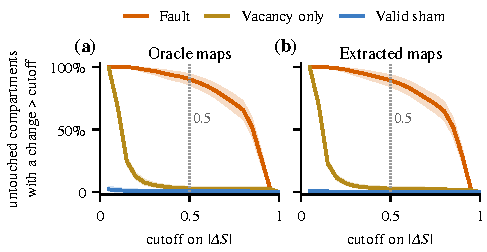
\includegraphics[width=.90\textwidth]{collateral.pdf}
\caption{\textbf{Collateral response across the sigmoid range.} For each fault, deletion, and sham we use the same 13 cells outside the donor and recipient cells. A cell contributes if at least one pixel reaches the specified absolute change. Shading shows original-image-paired 95\% intervals on each fraction. The maximum within a cell measures whether any pixel moves substantially.}
\label{fig:collateral}
\end{figure*}

\paragraph{Reference regions and scene operation.}
The two affected cells are a rule-based coarse spatial reference. The vacant and occupied cells need no pixel-level anomaly outline. For each cell we take the maximum of either the edited output or the absolute change from source. Even the change-based cell rank is 98.4\% on oracle maps while 90.3\% of untouched cells have a large absolute change. The matched deletion, which leaves the same vacancy, keeps changes above $0.5$ to 2.9\% of those same untouched cells. The paired difference is 87.4 points [82.4, 91.9] for oracle maps and 86.6 [81.4, 91.2] after extraction. \Cref{fig:collateral} shows the full threshold curve. These are changes in the spatial output, whereas scene-level maxima and cutoff decisions are a separate measurement.

The image score is the official maximum sigmoid output. The validation IQRs are 0.00974 (oracle) and 0.01060 (extracted). The raw cutoffs are 0.15802 and 0.17097. The rule comparator sums the absolute deviation from one pin per cell and adds retained out-of-grid pins. Its cutoff is zero on both paths. The comparator uses the same labels and the same validation rule. On re-extracted maps it yields zero sham alerts (exact 95\% upper bound 2.6\%), while retaining all 138 fault alerts. \Cref{tab:halves} reports the held-out halves and the paired effect. Figure selection uses the case closest to the median oracle fault-minus-sham score. There were zero missed faults. The second row uses the first hash-ordered alerted sham, whose source also alerts.

\begin{table*}[t]
\centering
\caption{\textbf{Held-out halves for the SALAD photo intervention.} Sham, Fault and Del. count alerts. All fault and deletion recalls are 100\% on the respective support. Bootstrap intervals for tied all-success contrasts are conditional on the sample.}
\label{tab:halves}
\scriptsize
\setlength{\tabcolsep}{3.3pt}
\begin{tabular}{@{}llrrrrrrr@{}}
\toprule
Maps & Split & Sources & Sham & Fault & Del. & Alarm gap (pp) & Paired wins (\%) & Comp. response AUROC \\
\midrule
Oracle & A & 63 & 15 & 63 & 63 & +76.2 [+65.1, +85.7] & 100.0 [100.0, 100.0] & 99.0 [98.4, 99.6] \\
Oracle & B & 75 & 16 & 75 & 75 & +78.7 [+69.3, +88.0] & 100.0 [100.0, 100.0] & 97.9 [96.3, 99.1] \\
Oracle & All & 138 & 31 & 138 & 138 & +77.5 [+70.3, +84.1] & 100.0 [100.0, 100.0] & 98.4 [97.5, 99.1] \\
\midrule
Extracted & A & 63 & 1 & 63 & 63 & +98.4 [+95.2, +100.0] & 100.0 [100.0, 100.0] & 99.2 [98.7, 99.6] \\
Extracted & B & 75 & 6 & 75 & 75 & +92.0 [+85.3, +97.3] & 100.0 [100.0, 100.0] & 98.1 [96.4, 99.1] \\
Extracted & All & 138 & 7 & 138 & 138 & +94.9 [+90.6, +98.6] & 100.0 [100.0, 100.0] & 98.6 [97.6, 99.2] \\
\bottomrule
\end{tabular}

\end{table*}

\subsection{Native LOCO and screw-bag follow-up}
The original SALAD repository checkpoint pair is used for each category. We verified the published download archive, the two checkpoint fingerprints per category, the upstream map decoder, and its unmodified composition forward pass. The maps are indexed labels, mapped to six channels without RGB conversion or interpolation. The expected output is a finite $256\times256$ array in $[0,1]$. In each category the same validation map repeated exactly. The code normalizes the maximum using its normal validation mean and standard deviation. A positive affine transform preserves all rankings and the corresponding validation-order-statistic threshold. The released inputs contain 1,778 fitting, 305 normal validation and 1,568 test entries. The original benchmark paper reports 1,772, 304 and 1,568. We retain the authors' archive splits and retain the authors' published full-system results as context for the original composition-only analysis \cite{fucka2025}.

\begin{table*}[t]
\centering
\caption{\textbf{Native map scores and composition branch alerts.} AUROC in percent. Pos/good counts positives and their eligible negative comparison images. Cutoffs come from normal validation only and stay fixed across scopes. Macro AUROC weights categories equally. Macro alert counts add images. Pushpins has no eligible matched signature.}
\label{tab:locodetail}
\scriptsize
\setlength{\tabcolsep}{4pt}
\begin{tabular}{@{}llrrrrrrrr@{}}
\toprule
Category & Scope & Pos/good & Bag & Grid & Pairs & Extent & SALAD [95\% CI] & Hits & Good alarms \\
\midrule
Breakfast box & Logical & 83/102 & 79.8 & 79.9 & 76.6 & 78.7 & 79.0 [71.6, 85.8] & 53/83 & 15/102 \\
 & Matched & 42/77 & 71.9 & 68.3 & 68.1 & 71.5 & 64.4 [53.4, 75.3] & 17/42 & 14/77 \\
 & Structural & 90/102 & 68.6 & 69.1 & 69.7 & 68.0 & 75.4 [68.2, 82.1] & 48/90 & 15/102 \\
\midrule
Juice bottle & Logical & 142/94 & 84.3 & 85.6 & 85.3 & 83.2 & 88.1 [83.5, 92.1] & 105/142 & 4/94 \\
 & Matched & 99/91 & 82.0 & 84.1 & 85.3 & 82.6 & 82.9 [77.0, 88.4] & 64/99 & 2/91 \\
 & Structural & 94/94 & 74.1 & 70.9 & 68.8 & 66.3 & 85.3 [79.5, 90.6] & 59/94 & 4/94 \\
\midrule
Pushpins & Logical & 91/138 & 77.2 & 76.9 & 73.3 & 67.1 & 99.7 [99.2, 100.0] & 91/91 & 31/138 \\
 & Structural & 81/138 & 56.1 & 59.8 & 53.7 & 50.0 & 76.4 [69.4, 82.9] & 47/81 & 31/138 \\
\midrule
Screw bag & Logical & 137/122 & 76.0 & 76.8 & 63.3 & 61.6 & 90.8 [86.6, 94.4] & 111/137 & 14/122 \\
 & Matched & 79/95 & 75.7 & 75.5 & 58.3 & 56.6 & 90.5 [85.1, 95.4] & 65/79 & 9/95 \\
 & Structural & 82/122 & 71.8 & 76.8 & 67.4 & 66.4 & 85.1 [79.3, 90.2] & 50/82 & 14/122 \\
\midrule
Connectors & Logical & 108/119 & 80.9 & 81.3 & 76.6 & 77.8 & 82.7 [76.8, 88.1] & 74/108 & 9/119 \\
 & Matched & 30/70 & 70.8 & 80.2 & 78.2 & 83.9 & 82.4 [74.6, 89.0] & 21/30 & 6/70 \\
 & Structural & 85/119 & 72.6 & 72.1 & 71.6 & 70.2 & 92.0 [87.8, 95.7] & 69/85 & 9/119 \\
\midrule
Macro & Logical & 561/575 & 79.6 & 80.1 & 75.0 & 73.7 & 88.1 [85.8, 90.2] & 434/561 & 73/575 \\
 & Matched & 250/333 & 75.1 & 77.0 & 72.5 & 73.7 & 80.0 [76.2, 83.8] & 167/250 & 31/333 \\
 & Structural & 432/575 & 68.6 & 69.7 & 66.2 & 64.2 & 82.8 [80.1, 85.4] & 273/432 & 73/575 \\
\bottomrule
\end{tabular}

\end{table*}

The native matched analysis uses the original component rule with an eight-connected minimum of 12 pixels, a catch-all class unseen in fitting, and both test labels plus at least five fitting maps in the signature. Each signature contributes a positive-weighted AUROC within category. The five-nearest-map baselines use blockwise standardized distances and the same training and calibration maps. Counts are per role. The part bag adds log total area and the median and range of log component areas. The grid adds fractional occupancy per role in a $4{\times}4$ grid. The pair block uses the mean coordinate offsets and the 10th, 50th and 90th percentiles of centroid distances by unordered role pair. It uses absolute coordinate offsets within a shared role. Distances are blockwise mean squared standardized differences with training-median imputation. Scale is $1.4826$ times the median absolute deviation, floored at 1.0, 0.25, 0.06 and 0.04 for counts, shapes, grid and pairs, respectively. Average the selected block distances before taking their square roots and averaging the five nearest maps. The extended pair variant uses the same counts and morphology. In the spatial block it averages the original pair distance with distances on absolute centroid position and shape. Position uses the 10th, 50th, and 90th percentiles of each coordinate by role. Extent pools log-transformed bounding spans and square roots of the two coordinate covariance eigenvalues at the same quantiles. The robust spread floors for these added blocks are 0.04 and 0.10. Defined coordinate features and fitted-median imputation follow the original procedure.

\begin{figure*}[t]
\centering
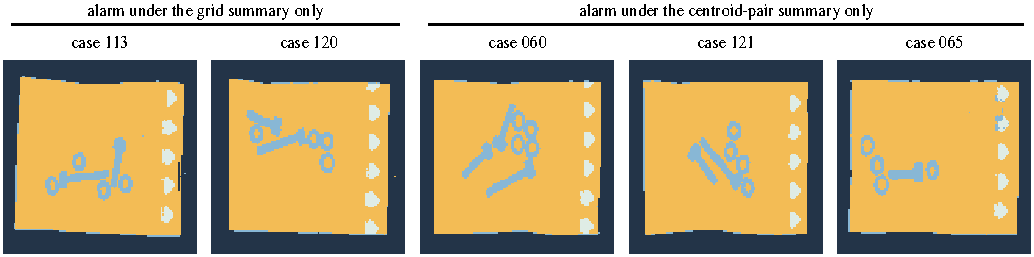
\includegraphics[width=.88\textwidth]{screw_discordant.pdf}
\caption{\textbf{Screw-bag logical cases with discordant grid and centroid-pair alerts.} At the locked thresholds, two of 79 supported faults alert under the grid alone and three under the pair summary alone. The colorized maps show the five cases. Thin fragments around the bag and merged foreground illustrate the difference between predicted counts and physical screw inventory.}
\label{fig:screw}
\end{figure*}

The matched screw-bag cohort has 79 faults and 95 good maps. Pairs trail the grid by 17.1 points [$-24.9$, $-9.0$] from unrounded scores (17.2 from rounded table entries). The other three categories average about $-0.3$ points. Adding placement and extent gives 56.6\% versus 58.3\% for the original pair block and 75.5\% for the grid. The paired difference relative to the original pair block is $-1.7$ points [$-9.9$, $+6.3$]. In \cref{fig:screw}, the predicted metal role includes narrow boundary fragments and can merge physical parts. For example, the largest projected long-axis extent in case 121 belongs to a 143-pixel fragment along the image-side edge. Per-role pooled extent therefore cannot identify the actual length of each screw. This probe supports a limit of the tested summaries on the supplied maps. In the native full comparison the grid's logical recall is 51.5\% macro with 11.1\% good alerts, versus 53.3\% and 10.3\% for the bag. Matched SALAD minus grid is $+3.0$ points [$-2.1$, $+8.2$] across the four supported categories and $+15.1$ [5.9, 24.5] in screw bag.

\subsection{One native SVC--PA query}
The code comparison keeps five negative fit patients, 20 negative calibration patients, and test patients with 24 Glenn codes and ten without. Mask face contact has 100\% test AUROC, detects 24/24 positives [85.8, 100], and alerts on 1/10 code-negative scans [0.25, 44.5]. The $31.47\,\mathrm{mm}^2$ calibration threshold is below the largest negative ($48.45$) and smallest positive ($58.17$). Axial-mask profiles detect 21/24 with zero negative alerts. Full contextual loss has 19.6\% AUROC and detects 0/24 at its cutoff. Its masked link probability is higher on the Glenn-coded test scans (median 0.712 versus 0.441). Refitting without the degree terms raises AUROC to 44.2\%. Removing the shared-neighbor terms gives 18.3\%. Distance alone gives 75.4\%. Removing one incident link at a time while holding the SVC--PA bit fixed yields mean absolute within-patient probability shifts of 0.093 on the 21 Glenn-coded patients with at least one such link and 0.144 on ten code-negative patients. These are exploratory sensitivity checks on five fit patients and a single query. They do not resolve the causal effects of surgery. Five target-negative SVC variants occur in the release, with two in fit and three in calibration. The test has zero. Independent adjudication of native relations and benign variants is needed to extend the scope beyond this code.



\section{Data use and review artifacts}
The medical experiments use existing de-identified research releases and reuse the original labels. This revision was a secondary analysis of those releases without new ethics review. There was no participant recruitment, intervention on people, or new consent collection for this secondary analysis. The HVSMR authors report approval by the Boston Children's Hospital IRB with a waiver of written consent \cite{pace2024}. The photographed assets derive from the public MVTec LOCO AD research dataset, distributed under CC BY-NC-SA 4.0. Derived image panels preserve that attribution and license. Analyses record the exact selected pairs, split assignments, scores, calibration rows, source and checkpoint hashes, and figure inputs. The protocol, scripts and verification receipts document the software and evidence trail.



\section*{LLM usage statement}
OpenAI Codex and Anthropic Claude were used to implement and run the experiments, check data and code provenance, generate figures and tables from saved outputs, and draft and edit the text. Every reported number is produced from saved outputs by scripts in the supplementary package.

{\small
\bibliographystyle{ieeenat_fullname}
\bibliography{references}
}
\end{document}
